\chapter{Evaluation}
\label{cha:evaluation}
\section{Experiment Environment}
\subsection{Compiler}
\label{section:compiler}
Minizinc IDE is a compiler which allows users to edit and run their models, which is developed by the University of Melbourne, Monash University, and Data61 Decision Sciences~\cite{r6}. It provides some build-in functions as well as optimization methods. In our models, the build-in Minizinc-to-Flatzinc translator and AC3 has been applied. In addition, A wide range of solvers has been tested~\cite{r6}.
\begin{itemize}
    \item Choco: A JAVA CSP solver, which supports many search strategies (DomWDeg, ABS, IBS, first-fail, etc.) and optimization processes (LNS, fast restart).
    \item Chuffed: A C++ FD solver using lazy clause generation, which contains a nogood logbook to avoid plenty of duplicate calculation.
    \item Coin-bc: A C++ based Mixed Integer Programming (in our case, the MIP model is the same with CSP model) solver, it adopts the branch and cut optimization.
    \item Gurobi: A commerical solver support MIP.
    \item Izplus: Based on iZ-C constraint programming that is developed by NTT DATA SEKISUI SYSTEMS CORPORATION. It combines Randomized restarting, Local search, Variable reordering and NG learning.
    \item Jacop: A JAVA CSP solver.
    \item Or-tool: An open-source solver developed by google, it combines many optimization methods.
    \item PicatSAT: A CSP solver based on picat which is a rule-based language. And it adopts log encoding~\cite{r8}.
    \item Yuck: Based on scala and combines local search with restarting, global constraints, and lexicographic cost functions.
\end{itemize}
\subsection{Software Platform}
\label{sec:softplat}
Most of experiments based on the Windows subsystem for Linux 2 (WSL2) which allows the developer run a Linux environment on Windows 10. Only the experiments related to izplus based on docker that is a lightweight virtual machine which applied container virtualization technology~\cite{r25}. Table~\ref{tab:Ubuntu} shows the version of the WSL2.
\begin{table*}[htbp]
  \centering

  \caption{The version of Windows subsystem for Linux}
  
  \label{tab:Ubuntu}
  \input table/Ubuntuversion.tex
\end{table*}
Furthermore, as mentioned in Chapter~\ref{section:compiler}, there are nine solvers has been applied in our experiment, Table~\ref{tab:solvers} indicates the version of each solver.
\begin{table}[htbp]
  \centering

  \caption{The solvers and corresponding versions}
  
  \label{tab:solvers}
  	\begin{subtable}[b]{\textwidth}
  	\centering
  \input table/solver1.tex
    \end{subtable}\\
    	\begin{subtable}[b]{\textwidth}
  	\centering
  \input table/solver2.tex
  \end{subtable}\\
  \begin{subtable}[b]{\textwidth}
  \centering
  \input table/solver3.tex
  \end{subtable}
\end{table}
\subsection{Hardware Platform}
\label{sec:hardplat}

\begin{table*}[htbp]
  \centering

  \caption{Processors used in our evaluation}
  
  \label{tab:machines}
  \input table/machines.tex
\end{table*}


\section{Result}
\label{sec:Result}
In this section, both the results of IQ Twist experiments and the results of Zig Zag Puzzler experiments will be discussed. Generally, all the cases in both games' booklets have been tested by the nine solvers. For each game, there are five difficulties 'start', 'junior', 'expert', 'master' and 'wizard'. Each difficulty consists of some cases. The time limit for running each case is 30 minutes, which is represented as 1800 seconds. If the solver can get the result in 1800 seconds, the time will be logged, otherwise, we treat it as a unsolved case. 
\\Above all, the discussions for the result will mainly include two parts, the coverage rates and the average time of each solver. For the coverage rates, it can be calculated by 
\begin{equation}
\label{equation:coverage}
   C= N1/N2\times 100\% ,
\end{equation}
where $C$ means the coverage rates, $N1$ means the number of solved cases and $N2$ means the number of total cases. And for the average time, it can be calculated by 
\begin{equation}
\label{equation:averagetime}
\overline{t}=\frac{\sum\limits_{i=1}^n t_{i}}{n},
\end{equation}
where $\overline{t}$ is the average execution time, $\sum\limits_{i=1}^n t_{i}$ is the sum of each execution time for solved cases and $n$ is the number of solved cases.
\subsection{IQ Twist Result}
\label{sec:IQtwistresult}
\begin{figure}[htbp]
    \centering
    \begin{subfigure}[b]{0.48\textwidth}
    \centering
    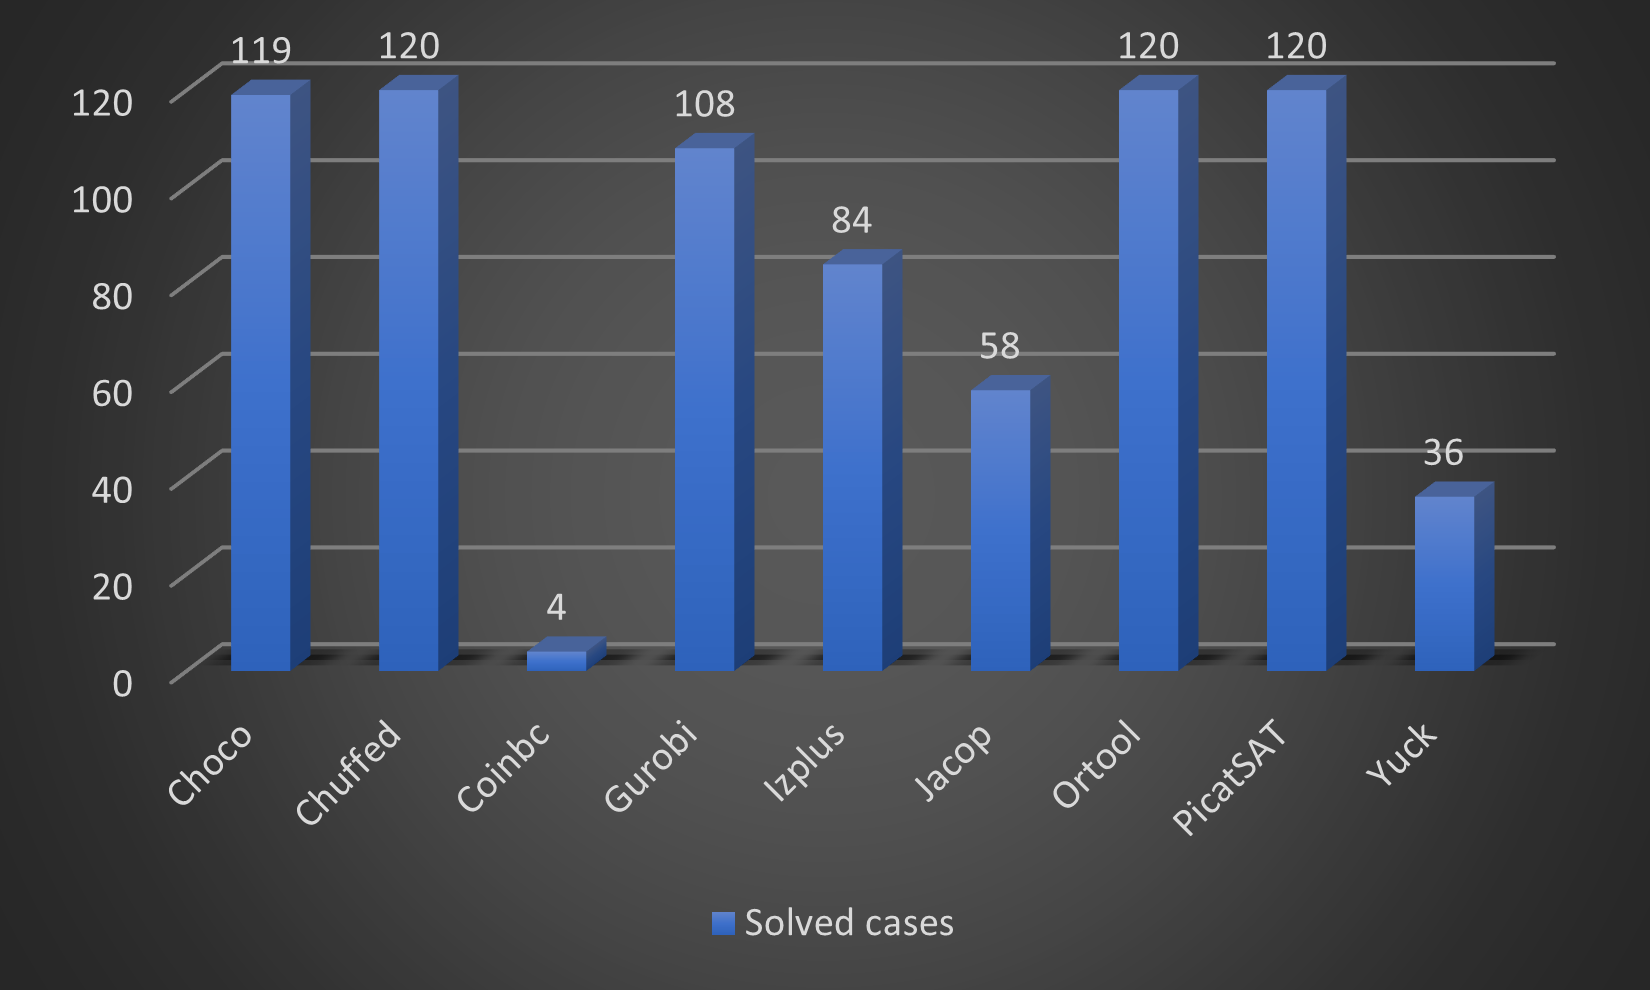
\includegraphics[width=\textwidth]{figs/solvedcases.png}
    \caption{The number of solved cases for each solver}
    \label{eva1}
    \end{subfigure}
     \begin{subfigure}[b]{0.48\textwidth}
     \centering
    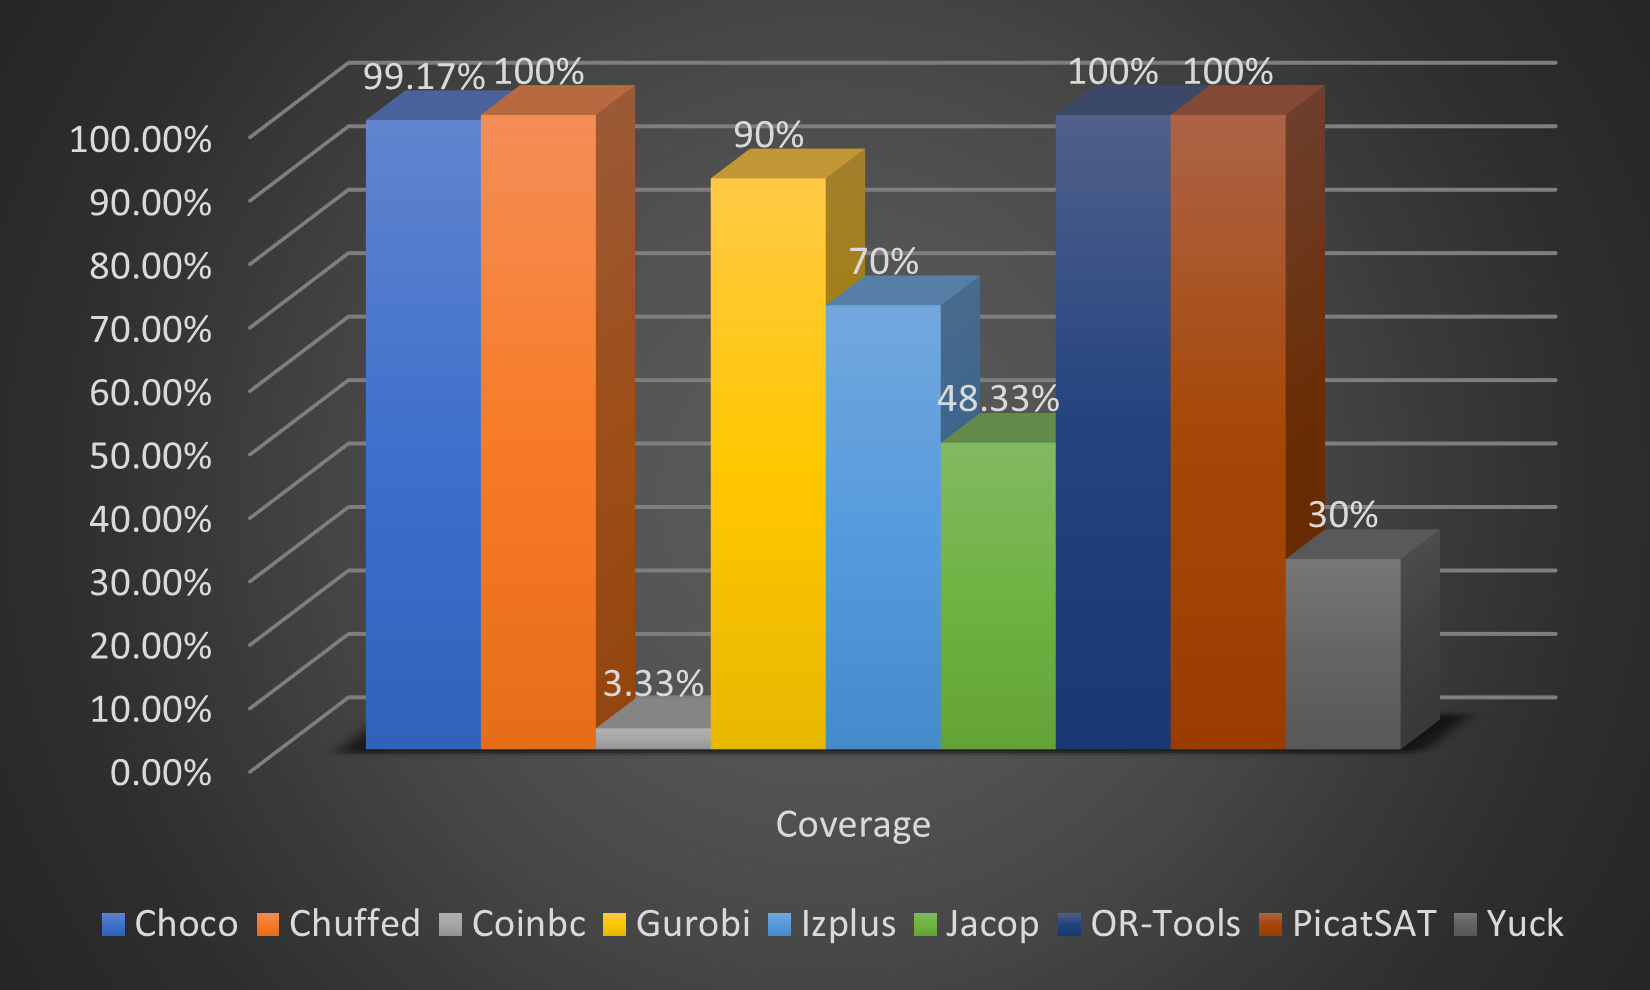
\includegraphics[width=\textwidth]{figs/coverage.png}
    \caption{Overall coverage rates of each solver}
    \label{eva2}
    \end{subfigure}
     \begin{subfigure}[b]{0.48\textwidth}
    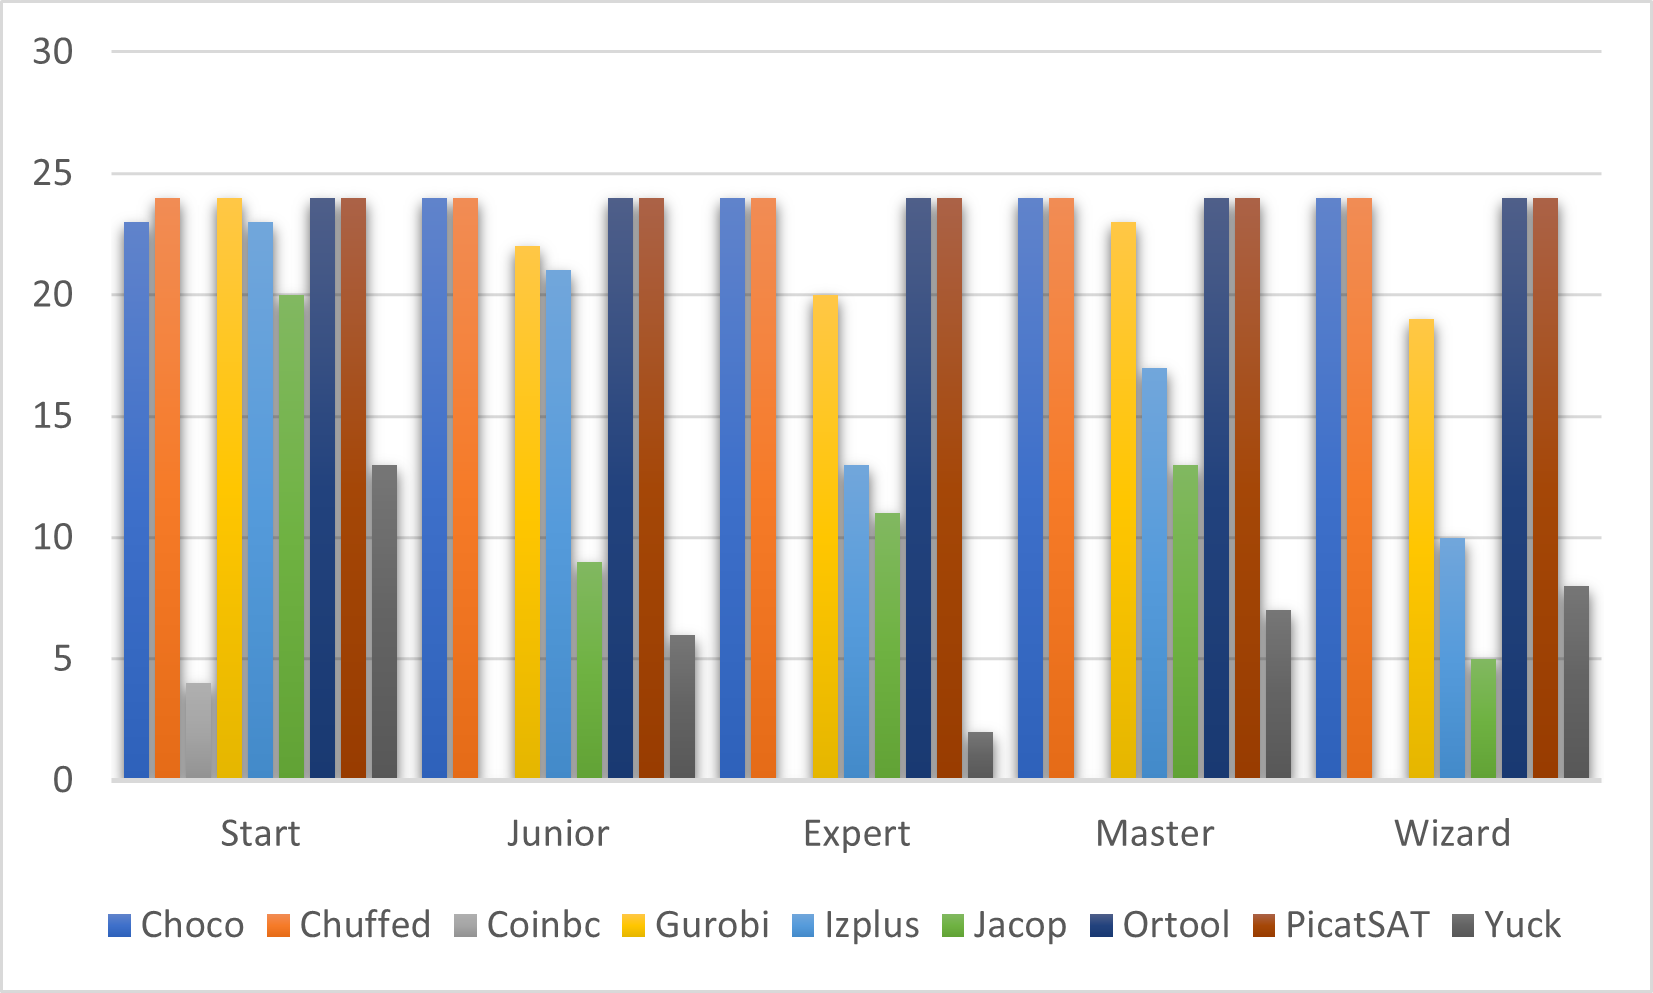
\includegraphics[width=\textwidth]{figs/separated number.png}
    \caption{The number of solved cases of each difficulty for each solver}
    \label{eva3}
    \end{subfigure}
    \begin{subfigure}[b]{0.48\textwidth}
    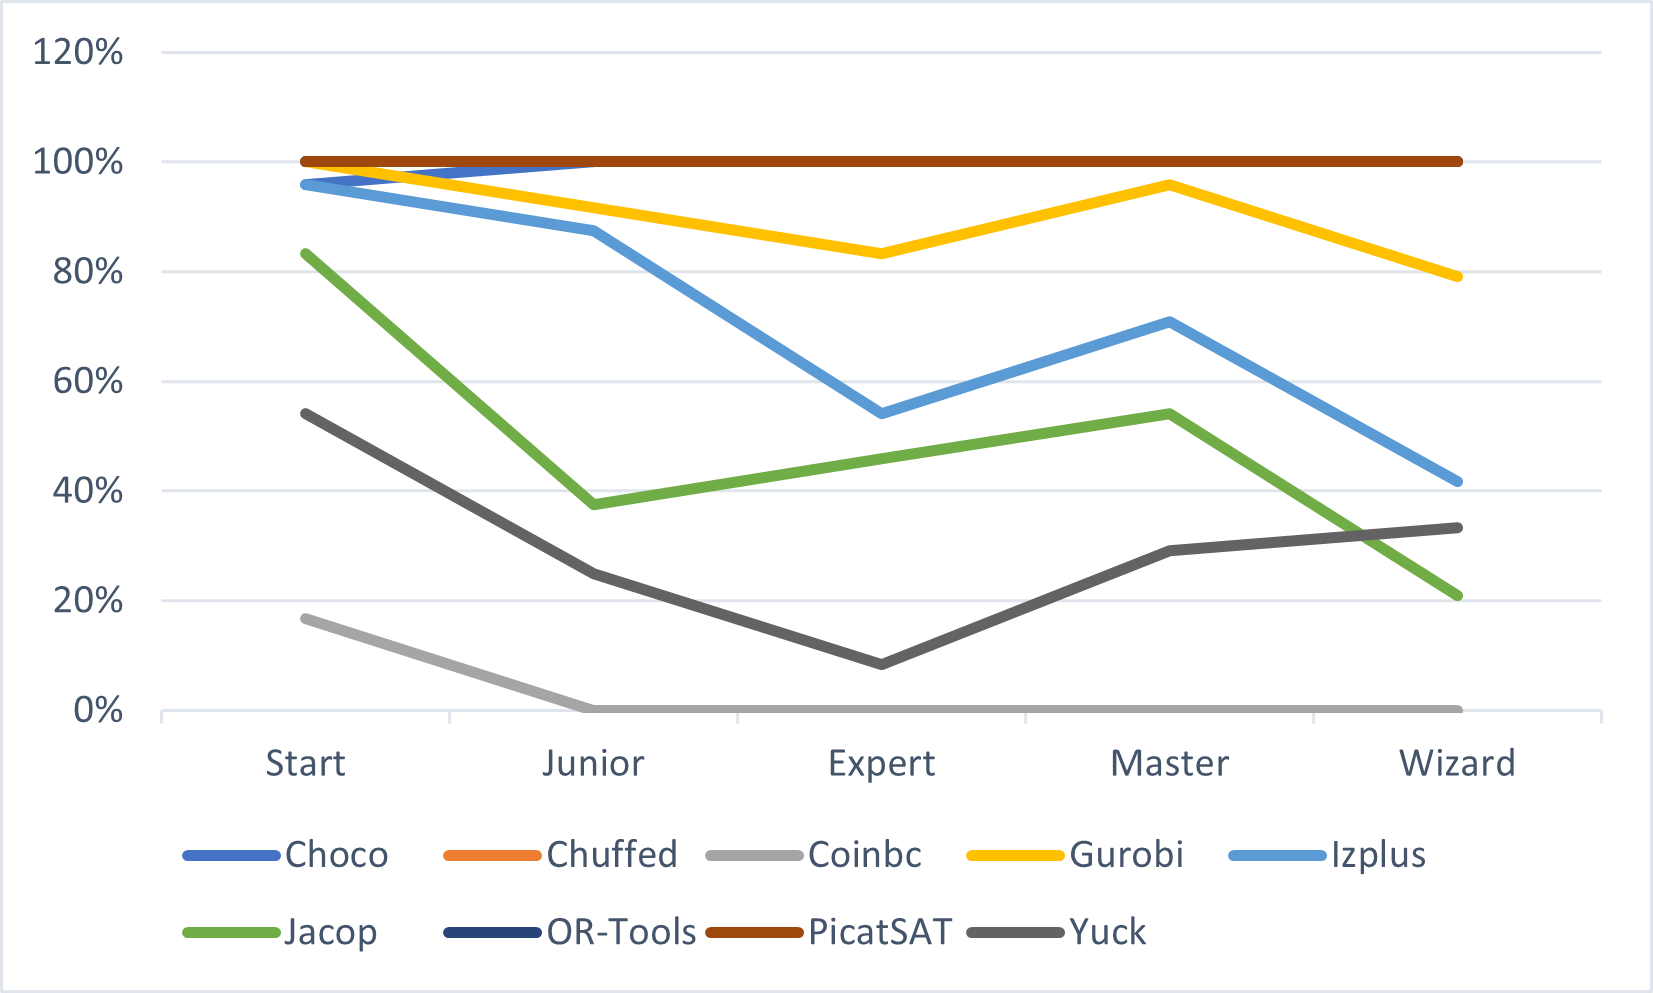
\includegraphics[width=\textwidth]{figs/separated coverage.png}
    \caption{The coverage rates of each difficulty for each solver}
    \label{eva4}
    \end{subfigure}
    \caption{Coverage rates and the number of solved cases in IQ Twist}
    \label{fig:comparisonIQtwist}
\end{figure}
In IQ twist booklet, there is a total of 120 cases, every 24 cases make up a difficulty.
Firstly, for each solver, we can calculate the coverage rates by the Equation~\ref{equation:coverage}.
Figure~\ref{eva1} shows the overall solved cases for each solver. Based on the data in Figure~\ref{eva1}, Figure~\ref{eva2} shows the overall coverage rates for different solvers, which indicates that there are only 3 solvers' overall coverage rates are 100 percentage. In addition, Figure~\ref{eva3} separately shows the solved cases of different difficulties for each solver. Accordingly, Figure~\ref{eva4} illustrates the change of coverage rates as the increasing of difficulty. It seems like that the other solvers are not stable in different difficulties except there are 3 solvers which always keep 100 percentages. Therefore, compared with other solvers, picatSAT, ortool and chuffed take advantages in coverage rates.
\\In addition, based on the solved cases, we calculate the average execution time for each solver by Equation~\ref{equation:averagetime}.
\begin{figure}[htbp]
\centering
\begin{subfigure}{0.48\textwidth}
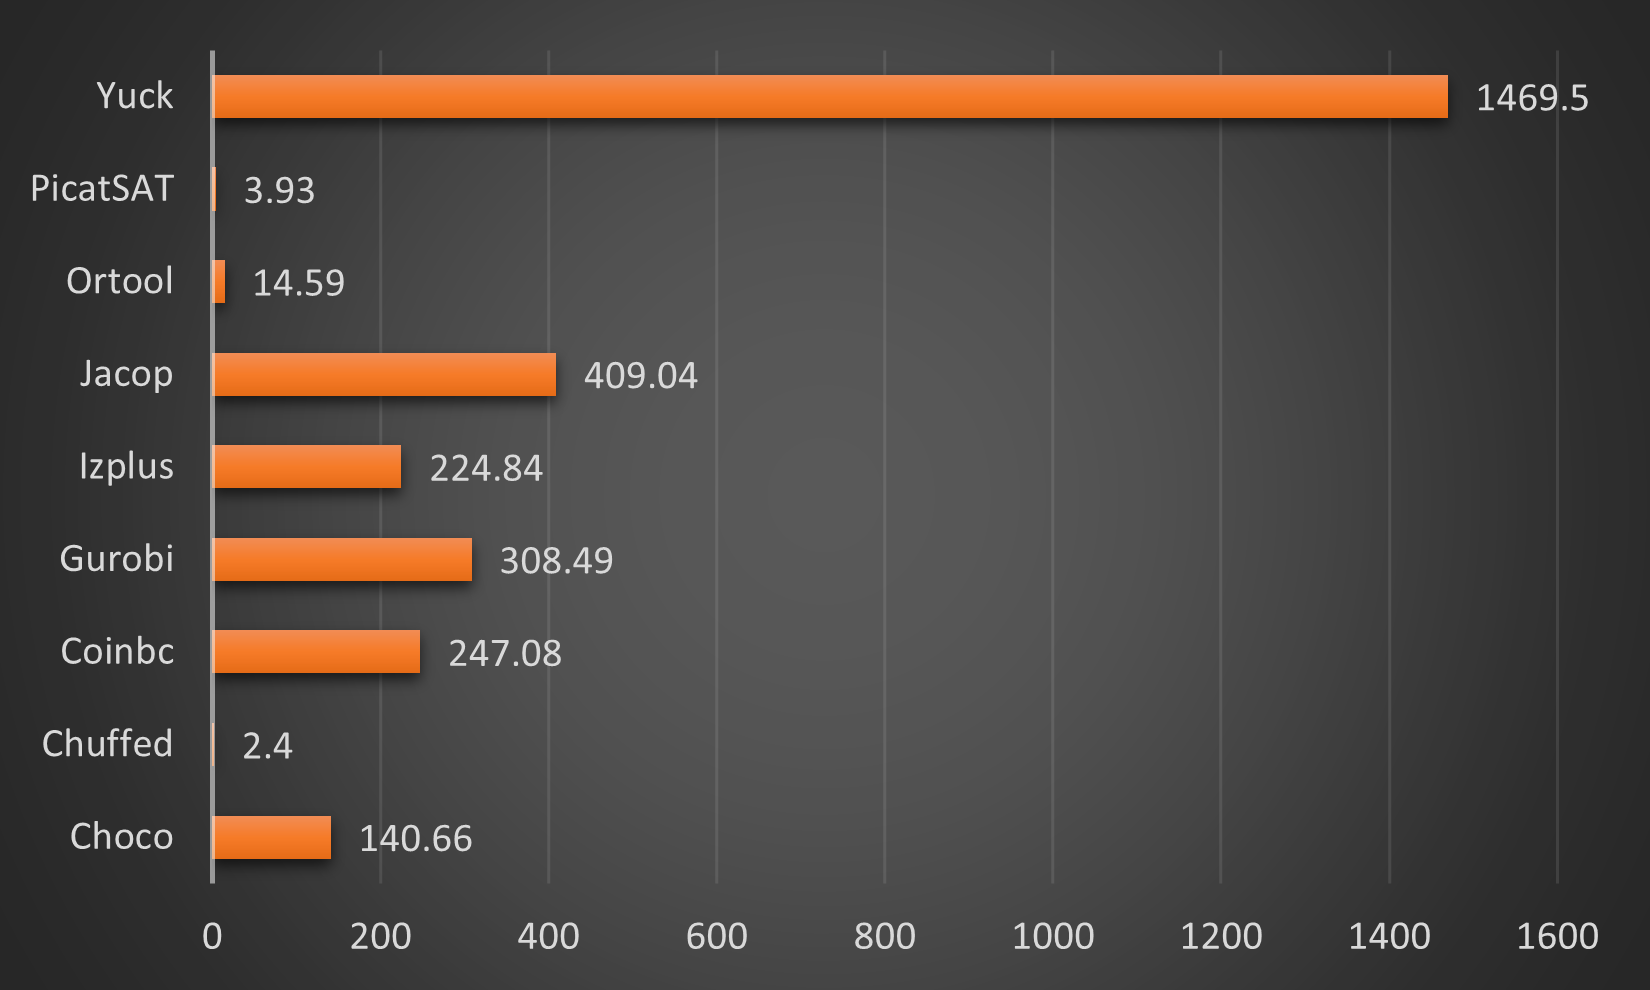
\includegraphics[width=\textwidth]{figs/averagetime.png}
\caption{The overall average execution time for solved cases}
\label{fig:averagetime1}
\end{subfigure}
\begin{subfigure}{0.48\textwidth}
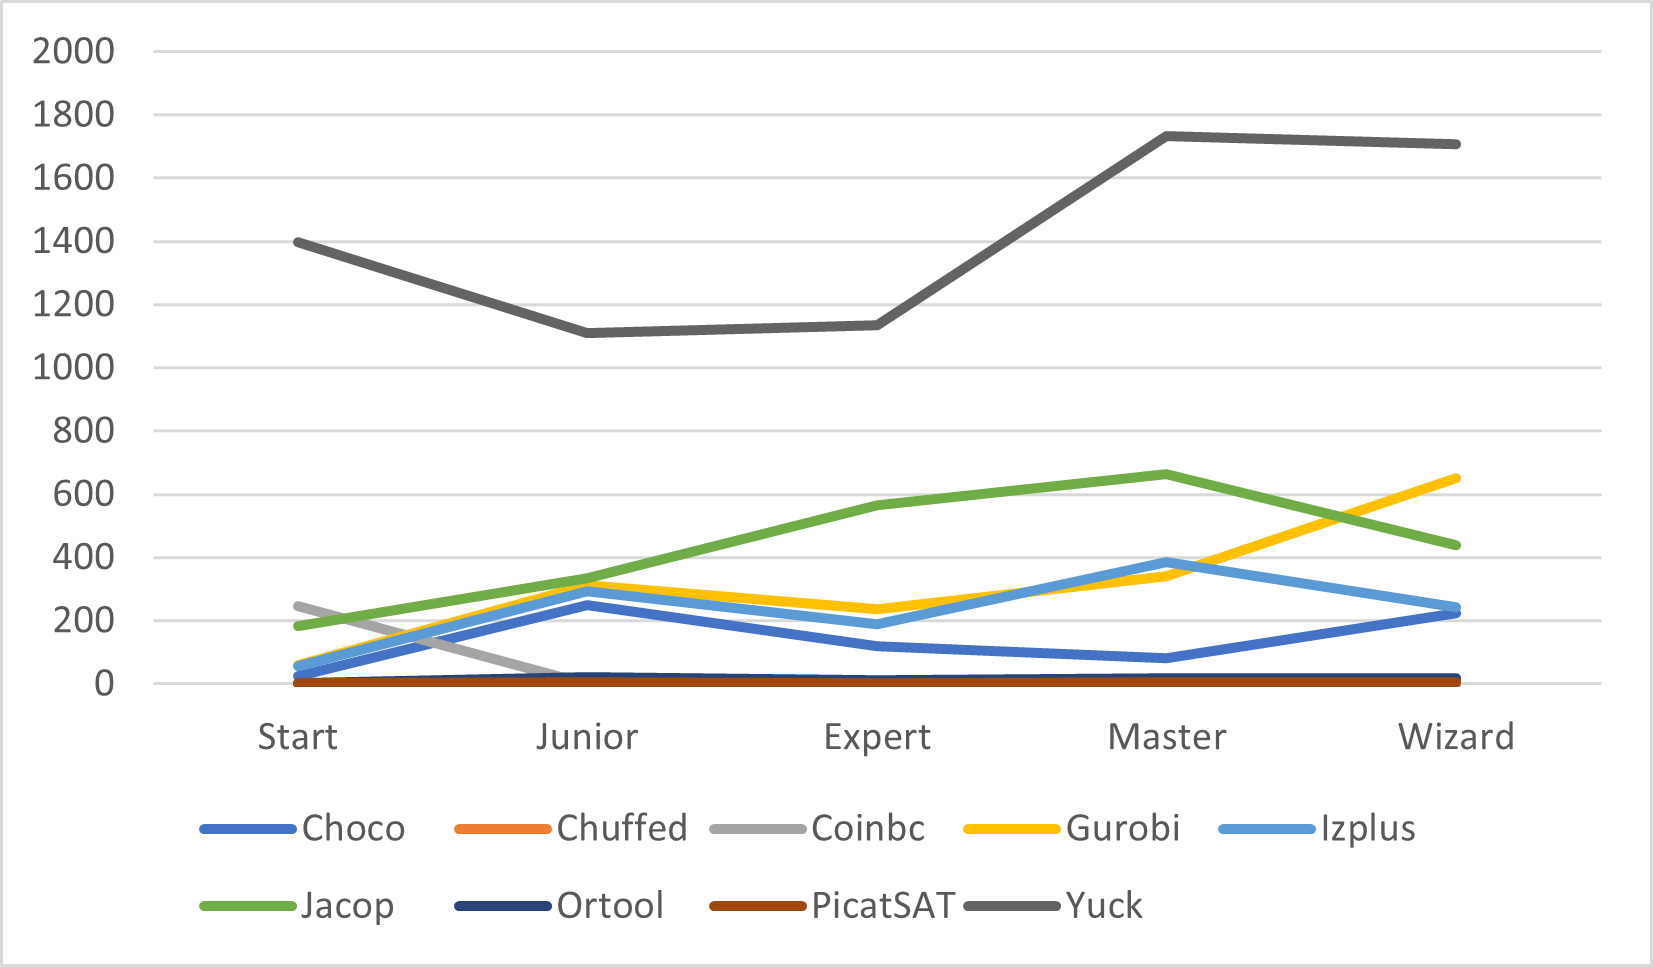
\includegraphics[width=\textwidth]{figs/separated time.png}
\caption{The separated average execution time for solved cases}
\label{fig:averagetime2}
\end{subfigure}
\caption{The average execution time for solved cases}
\label{fig:averagetime}
\end{figure}
Figure~\ref{fig:averagetime1} shows the overall average execution time for each solver. Again, chuffed, picatSAT and ortool takes huge advantages compared with other solvers. More specifically, the overall execution times of chuffed and picatSAT are close, and they are better than the overall execution time of Ortool. In addition, in Figure~\ref{fig:averagetime2}, the average time is 1800 seconds means the solvers can't solver any models in such a difficulty. Obviously, it indicates that the coin-bc can only solve the cases in the "start" level.
\begin{figure}[htbp]
\centering
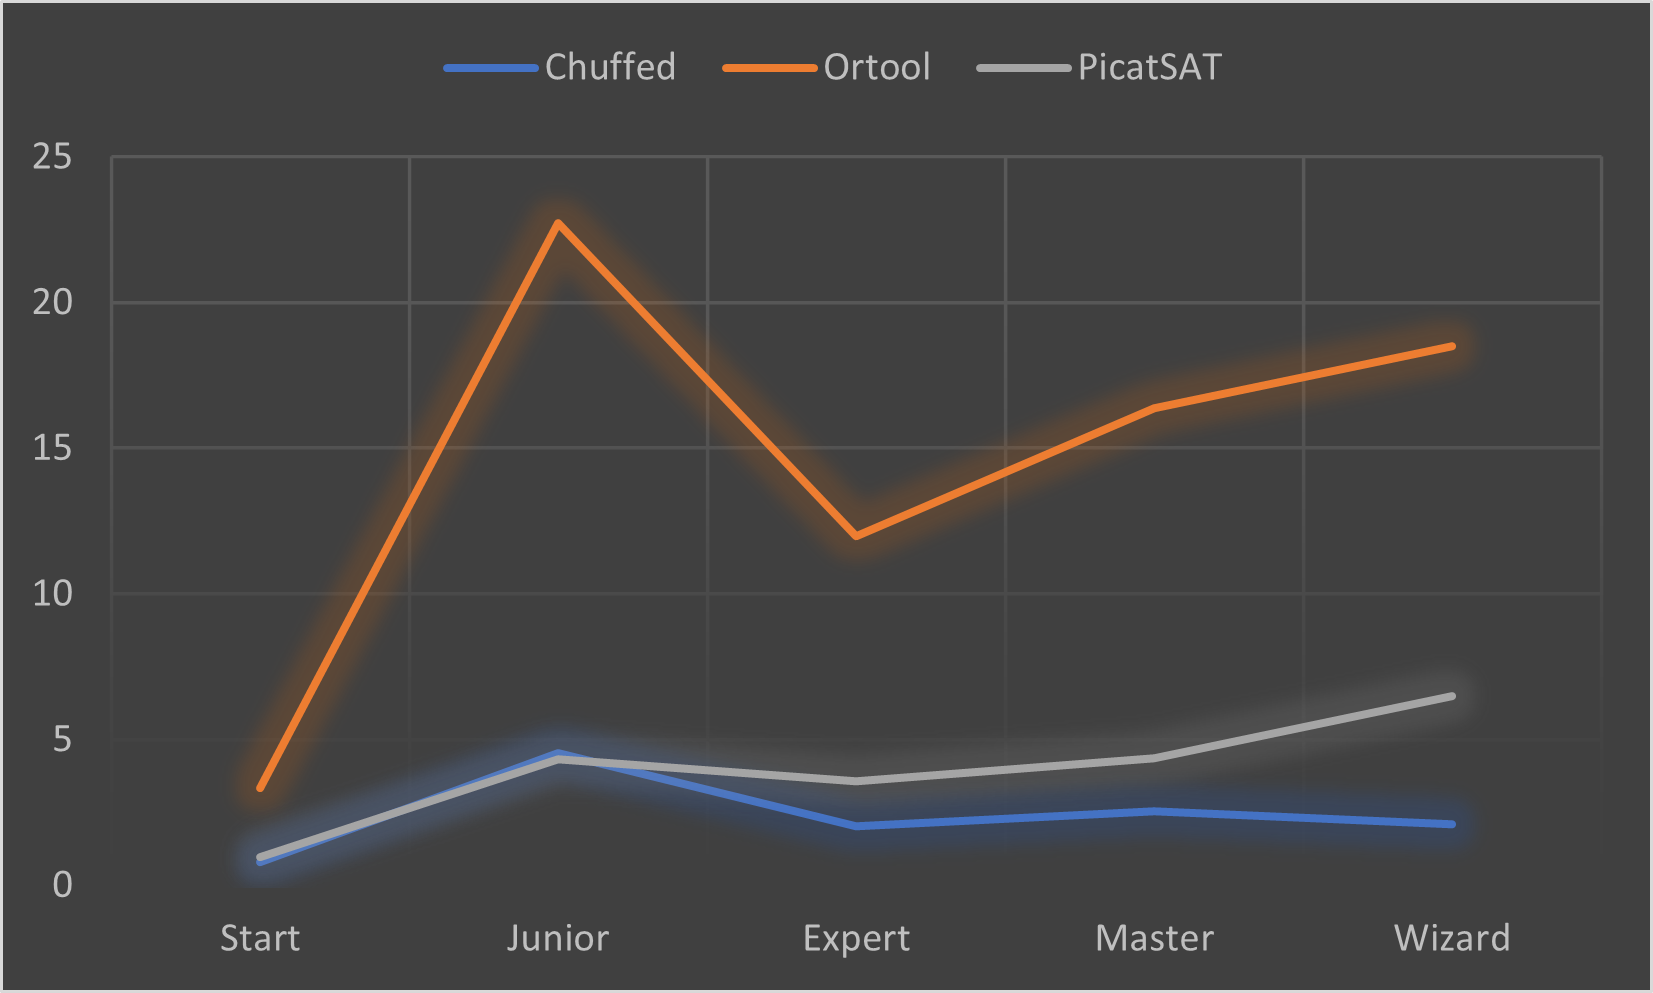
\includegraphics[width=0.6\textwidth]{figs/Three comparison.png}
\caption{The separated execution time comparisons between chuffed, picatSAT and ortool}
\label{fig:3comparison}
\end{figure}
Furthermore, Figure~\ref{fig:3comparison} indicates that the chuffed spends less time than picatSAT except in the "junior" difficulty.
\\Overall, although all of chuffed, picatSAT and ortool can get the result for each case in 30 minutes, the Chuffed possesses the best performance in IQ Twist.
\subsection{Zig Zag Puzzler Result}
\label{sec:Zig Zag Puzzlerresult}
In Zig Zag Puzzler booklet, there is a total of 80 cases, 40 of them belong to playing mode1, and the other 40 belong to playing mode2. For each playing mode, every 8 cases make up a difficulty. 
\subsubsection{Playing Mode1}
\begin{figure}[htbp]
    \centering
    \begin{subfigure}[b]{0.48\textwidth}
    \centering
    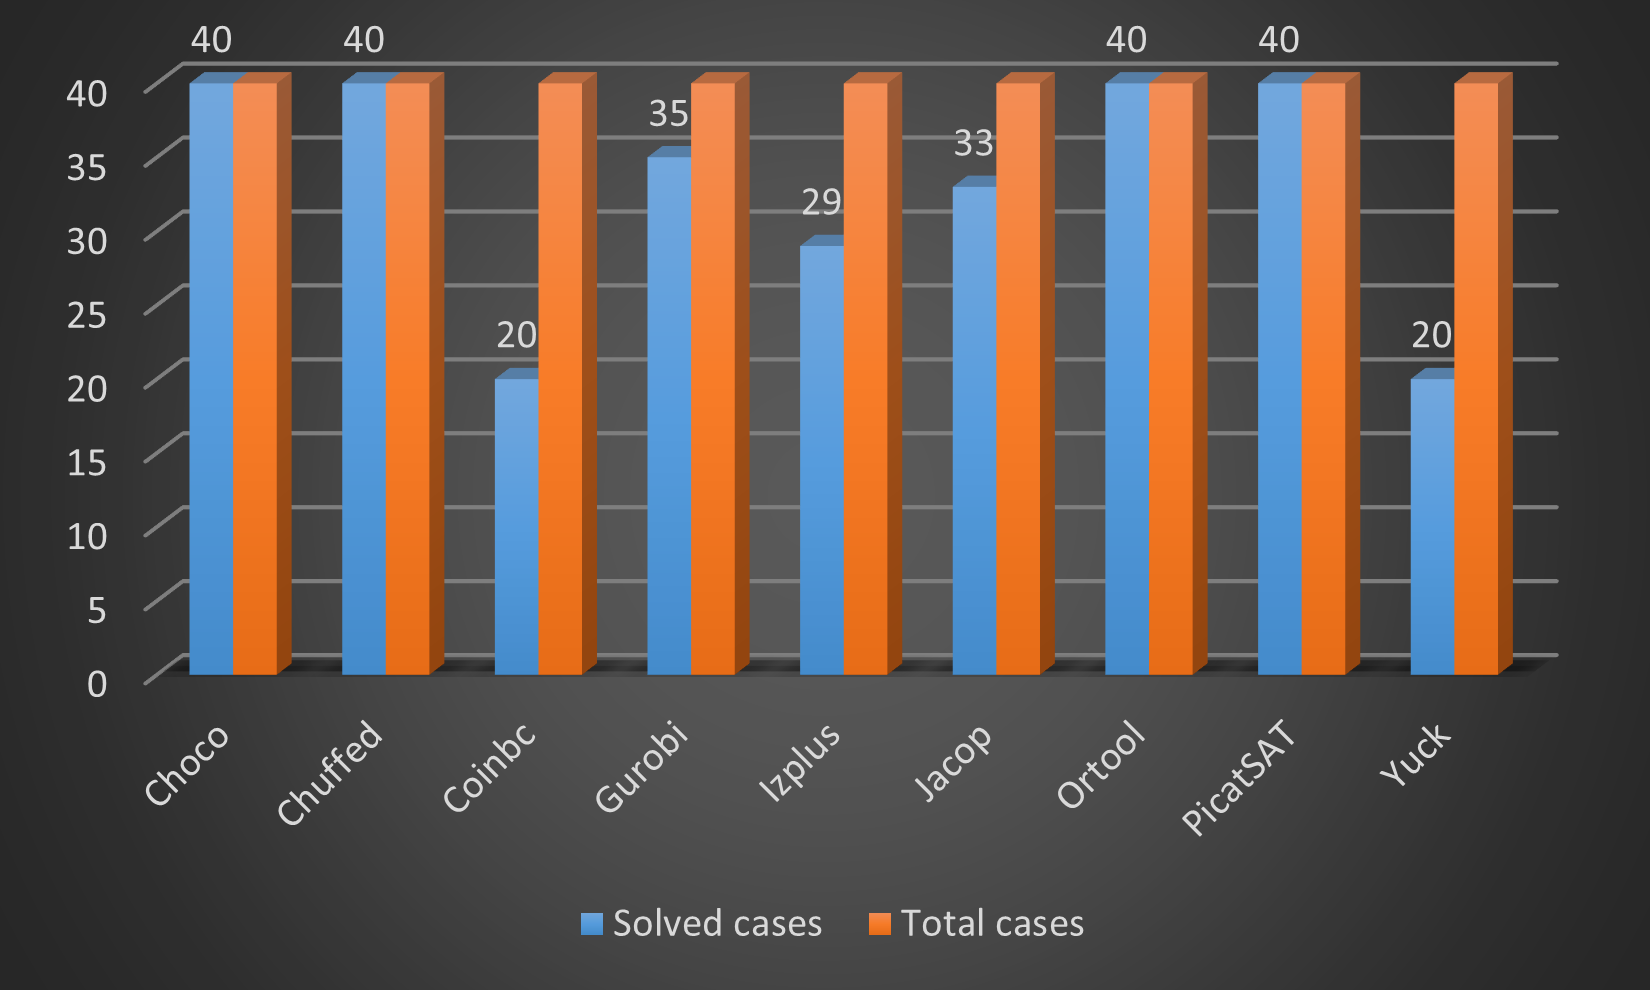
\includegraphics[width=\textwidth]{figs/mode1solvedcases.png}
    \caption{The number of solved cases for each solver}
    \label{fig:mode1eva1}
    \end{subfigure}
     \begin{subfigure}[b]{0.48\textwidth}
     \centering
    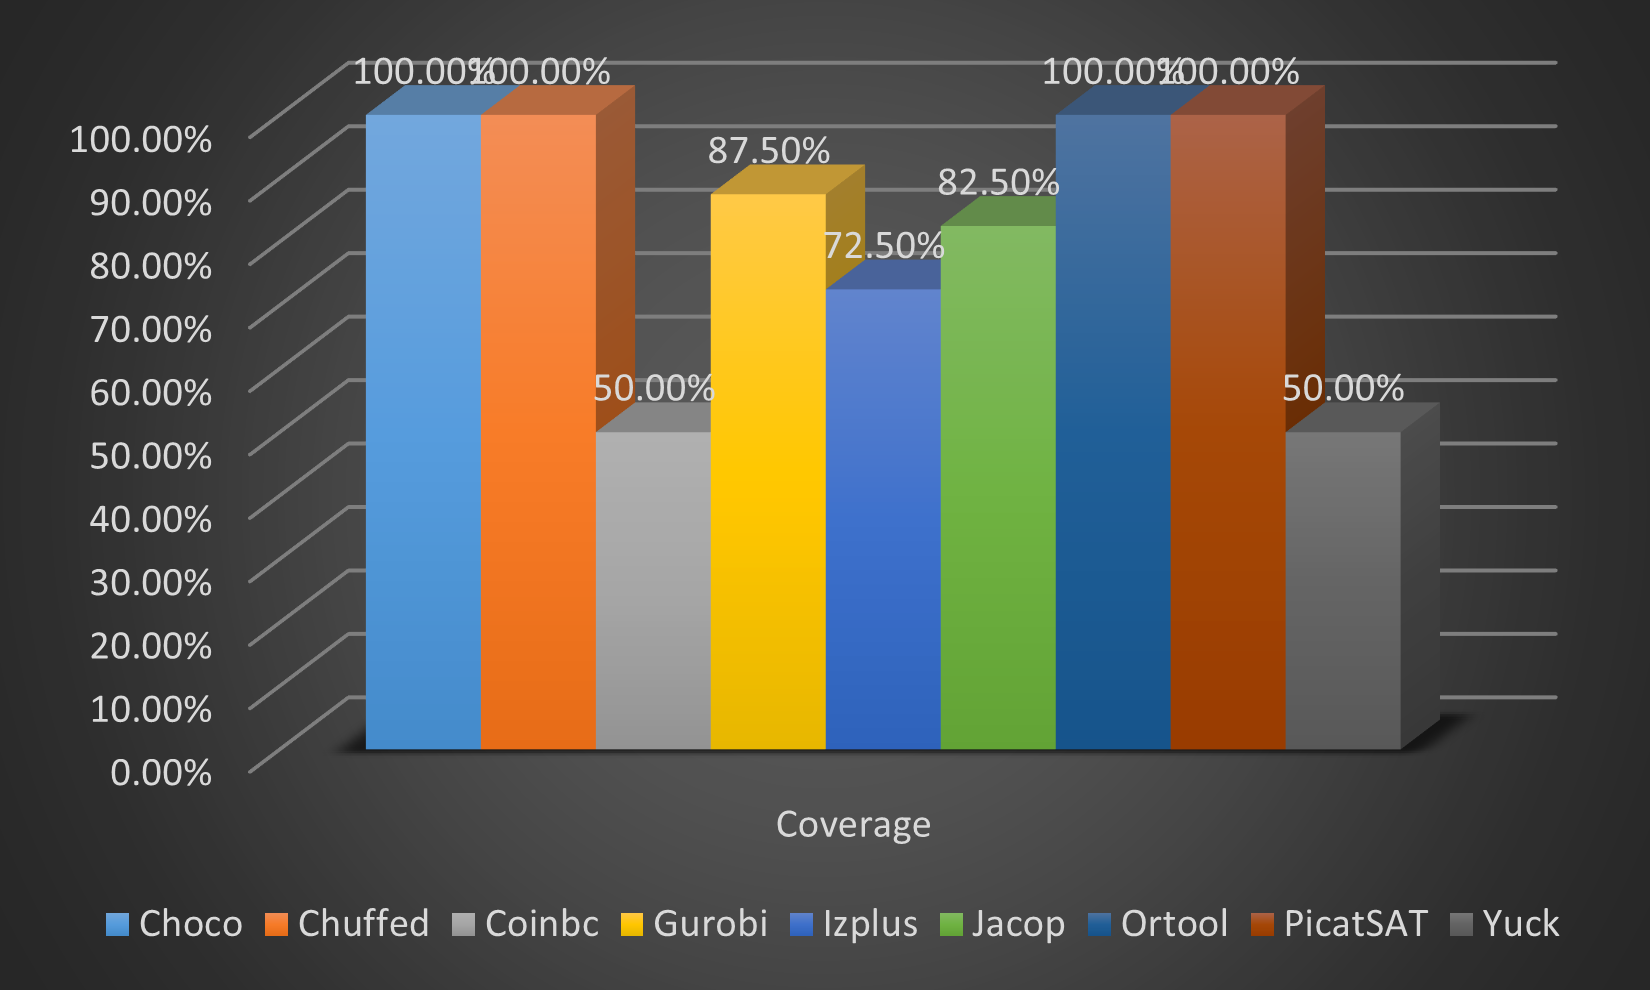
\includegraphics[width=\textwidth]{figs/mode1coverage.png}
    \caption{Overall coverage rates of each solver}
    \label{fig:mode1eva2}
    \end{subfigure}
     \begin{subfigure}[b]{0.48\textwidth}
    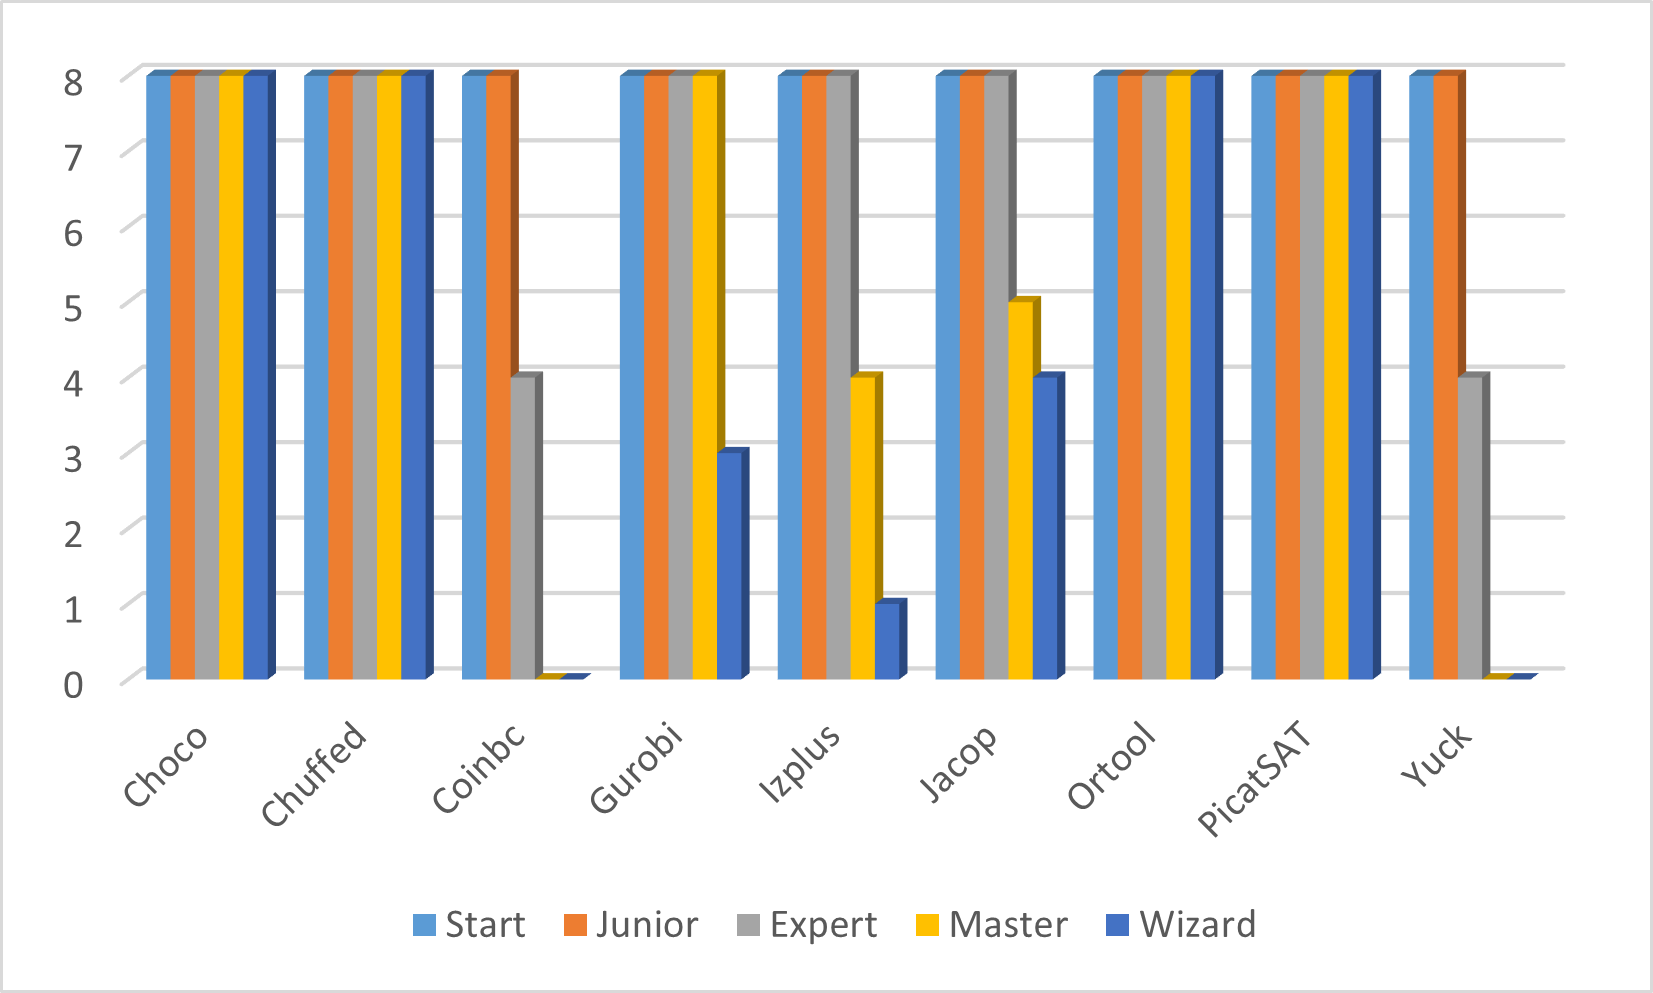
\includegraphics[width=\textwidth]{figs/mode1seperatedcases.png}
    \caption{The number of solved cases of each difficulty for each solver}
    \label{fig:mode1eva3}
    \end{subfigure}
    \begin{subfigure}[b]{0.48\textwidth}
    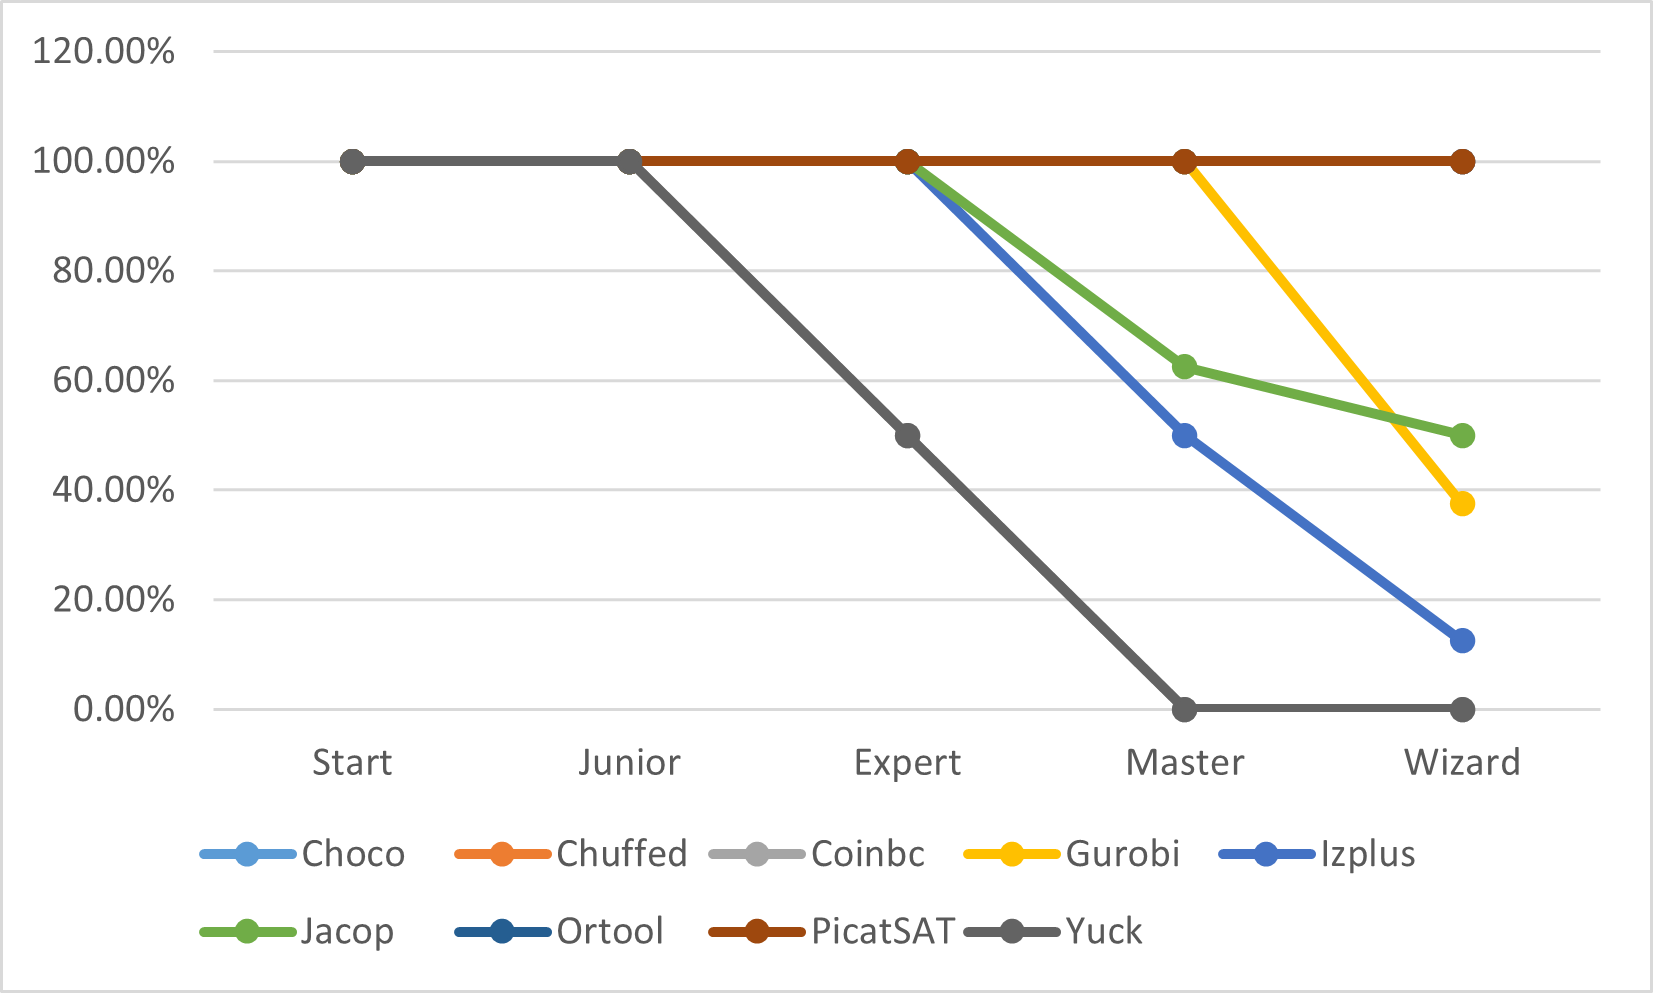
\includegraphics[width=\textwidth]{figs/mode1seperatedcoverage.png}
    \caption{The coverage rates of each difficulty for each solver}
    \label{fig:mode1eva4}
    \end{subfigure}
    \caption{Coverage rates and the number of solved cases in Zig Zag Puzzler playing mode1}
    \label{fig:comparisonmode1}
\end{figure}
Firstly, for each solver, we can calculate the coverage rates by the Equation~\ref{equation:coverage}. According to the data in Figure~\ref{fig:mode1eva1}, Figure~\ref{fig:mode1eva2} indicates that there are 4 solvers keep 100 percentages in the overall coverage. In addition, Figure~\ref{fig:mode1eva4} reveals that the other 5 solvers' separated coverage are decreased as the difficulty increase. 
\begin{figure}[htbp]
\centering
\begin{subfigure}{0.48\textwidth}
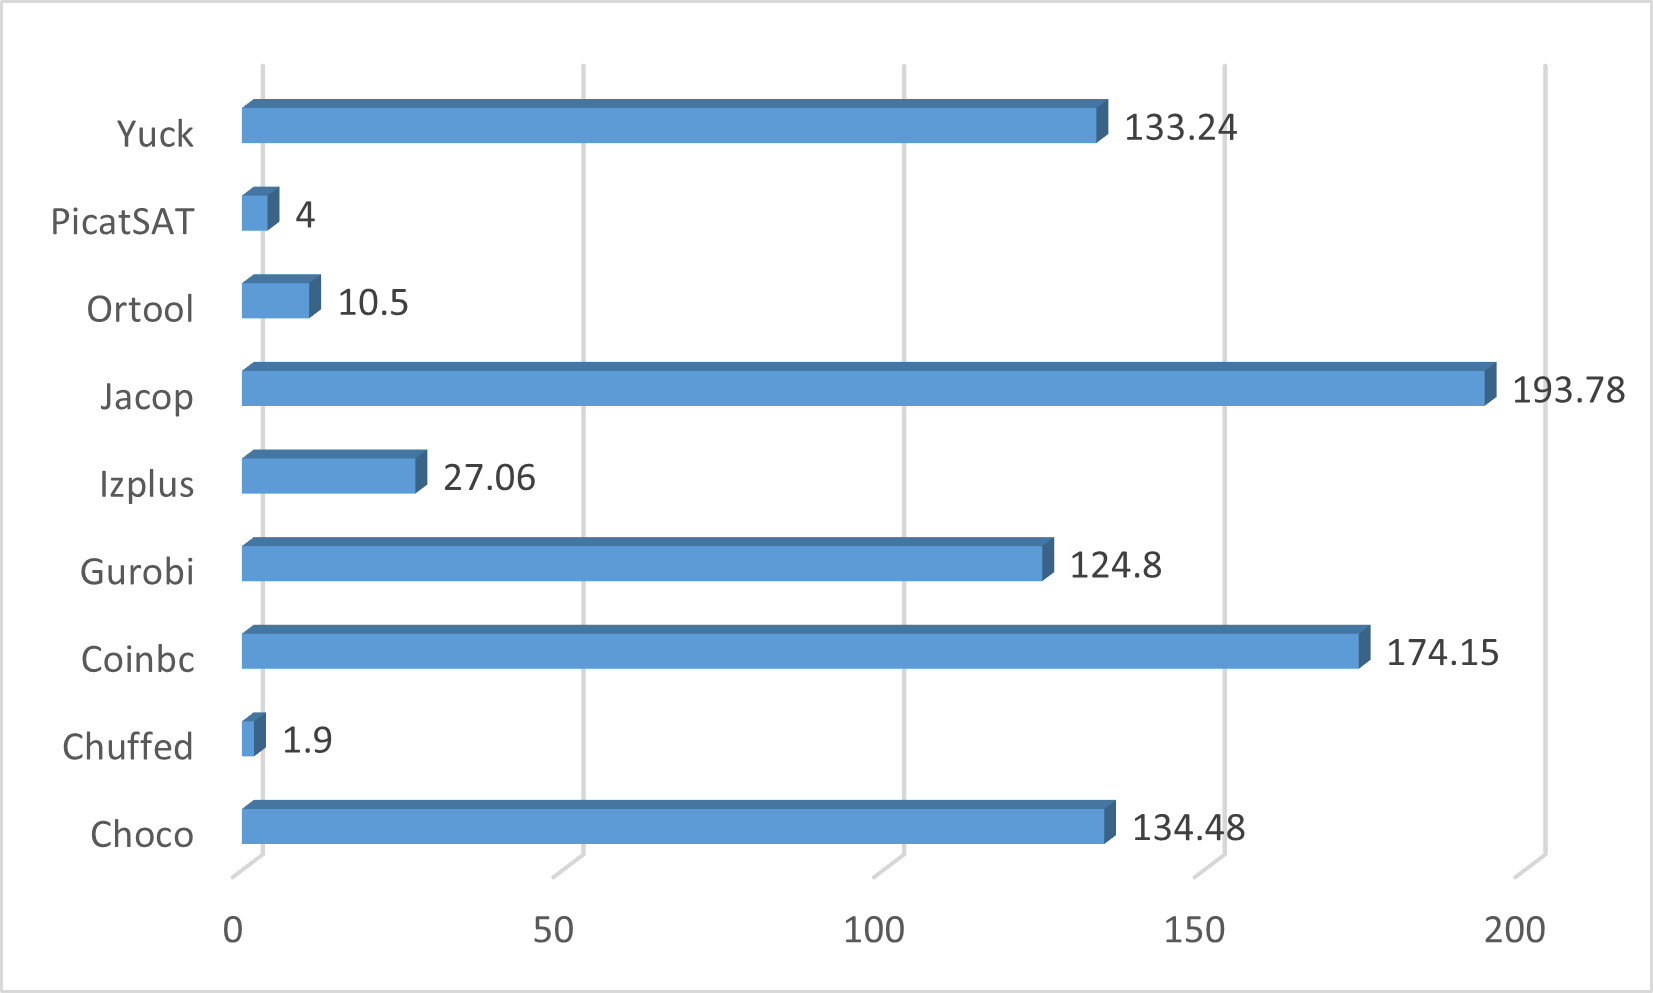
\includegraphics[width=\textwidth]{figs/mode1averagetime.png}
\caption{The overall average execution time of solved cases}
\label{fig:mode1averagetime1}
\end{subfigure}
\begin{subfigure}{0.48\textwidth}
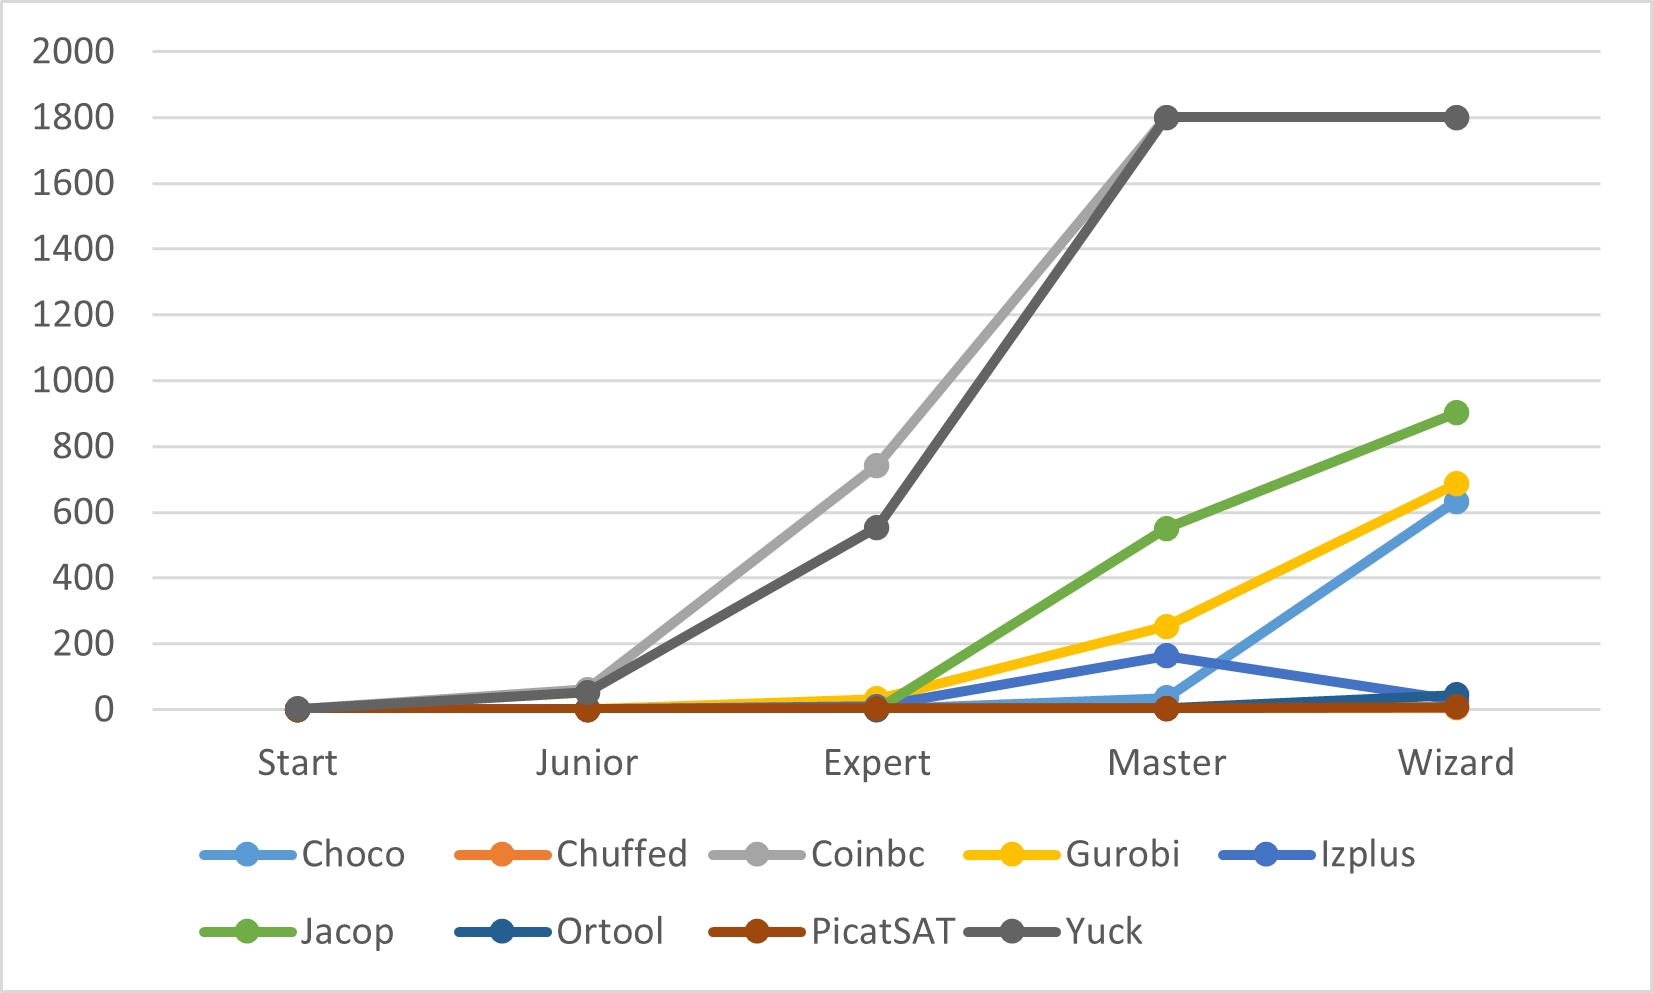
\includegraphics[width=\textwidth]{figs/mode1seperatedtime.png}
\caption{The separated average execution time of solved cases}
\label{fig:mode1averagetime2}
\end{subfigure}
\caption{The average execution time of solved cases}
\label{fig:mode1averagetime}
\end{figure}
For the average execution time, Figure~\ref{fig:mode1eva2} and Figure~\ref{fig:mode1averagetime1} illustrate that except Choco, the other 3 solvers which contain 100 percentages overall coverage rates need shorter overall average execution time too. For Choco, even though it solves every case in 30 minutes, its performance in overall average execution time is poor. And Figure~\ref{fig:compare} reveals that although the start point is very close, the growth rate of slopes for chuffed is much solver than ortool and picatSAT. Meanwhile, Figure~\ref{fig:mode1averagetime2} reveals a obvious positive correlation between the average execution time of different solvers and the difficulties except the curve of izplus. Based on Figure~\ref{fig:compare} and Figure~\ref{fig:mode1averagetime2}, chuffed has the optimal performance because of the lowest growth rate of slopes. 
\begin{figure}[htbp]
    \centering
    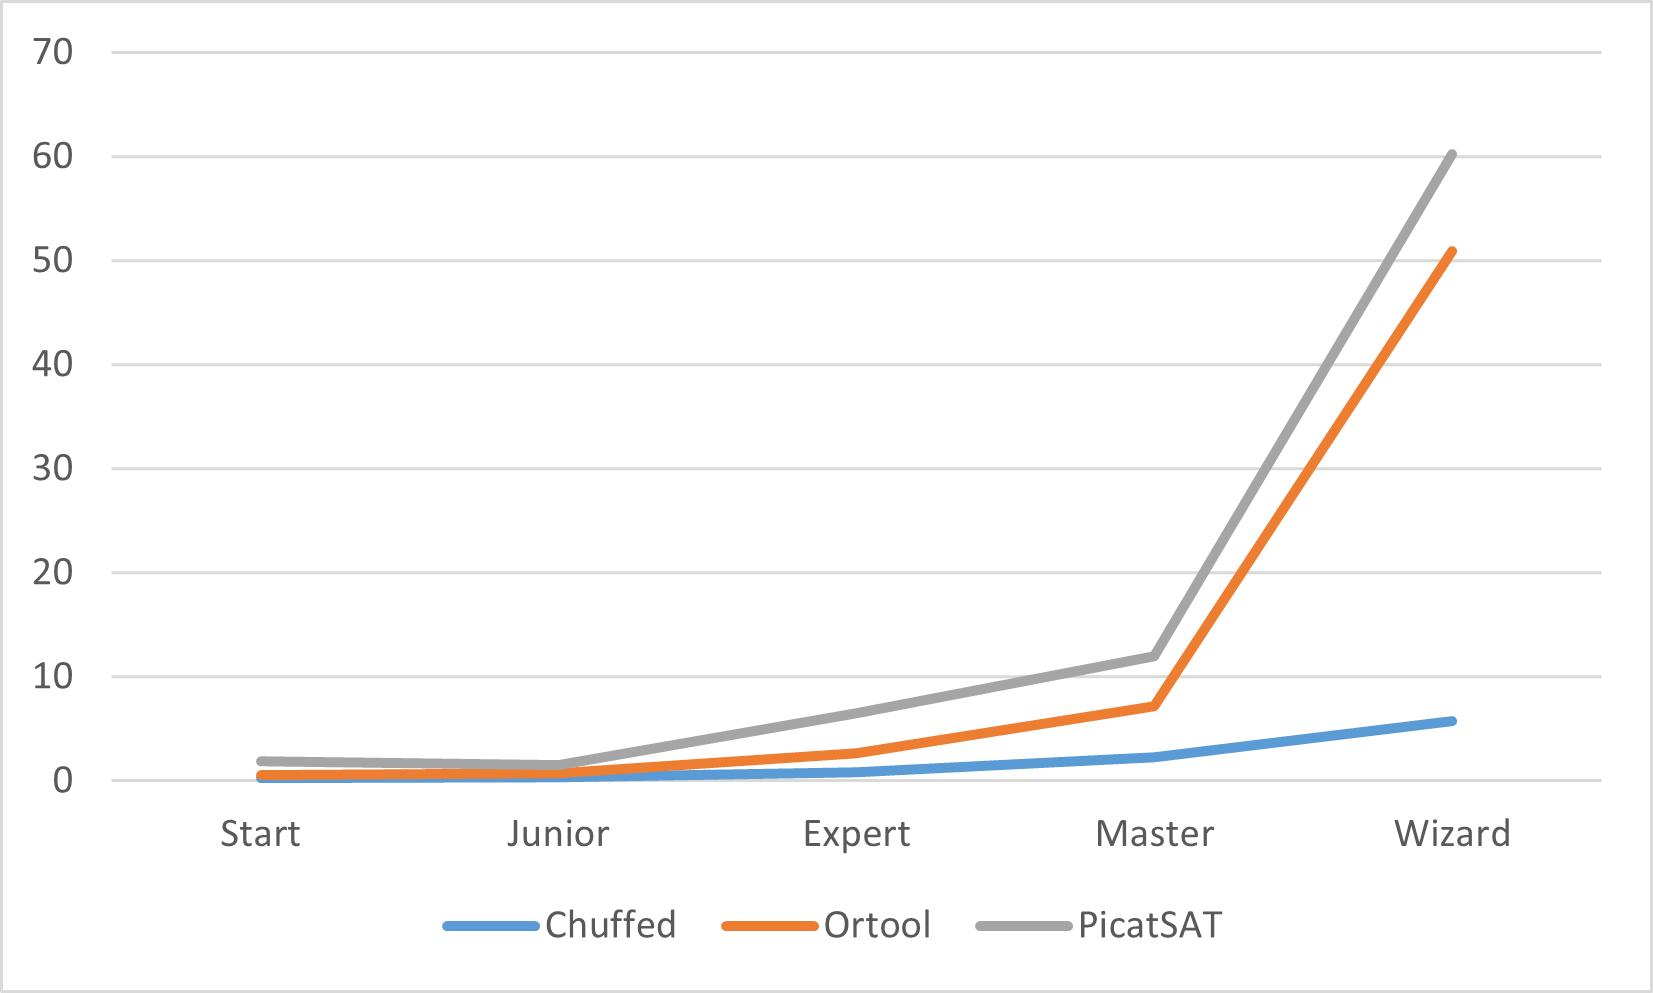
\includegraphics[width=0.6\textwidth]{figs/mode1solverscomparison.png}
    \caption{The separated average execution time of solved cases for chuffed, ortool and picatSAT}
    \label{fig:compare}
\end{figure}
Overall, combine coverage and average execution time, chuffed possess the best performance in Zig ZAG Puzzler playing mode1.
\subsubsection{Playing Mode2}
\begin{figure}[htbp]
    \centering
    \begin{subfigure}[b]{0.48\textwidth}
    \centering
    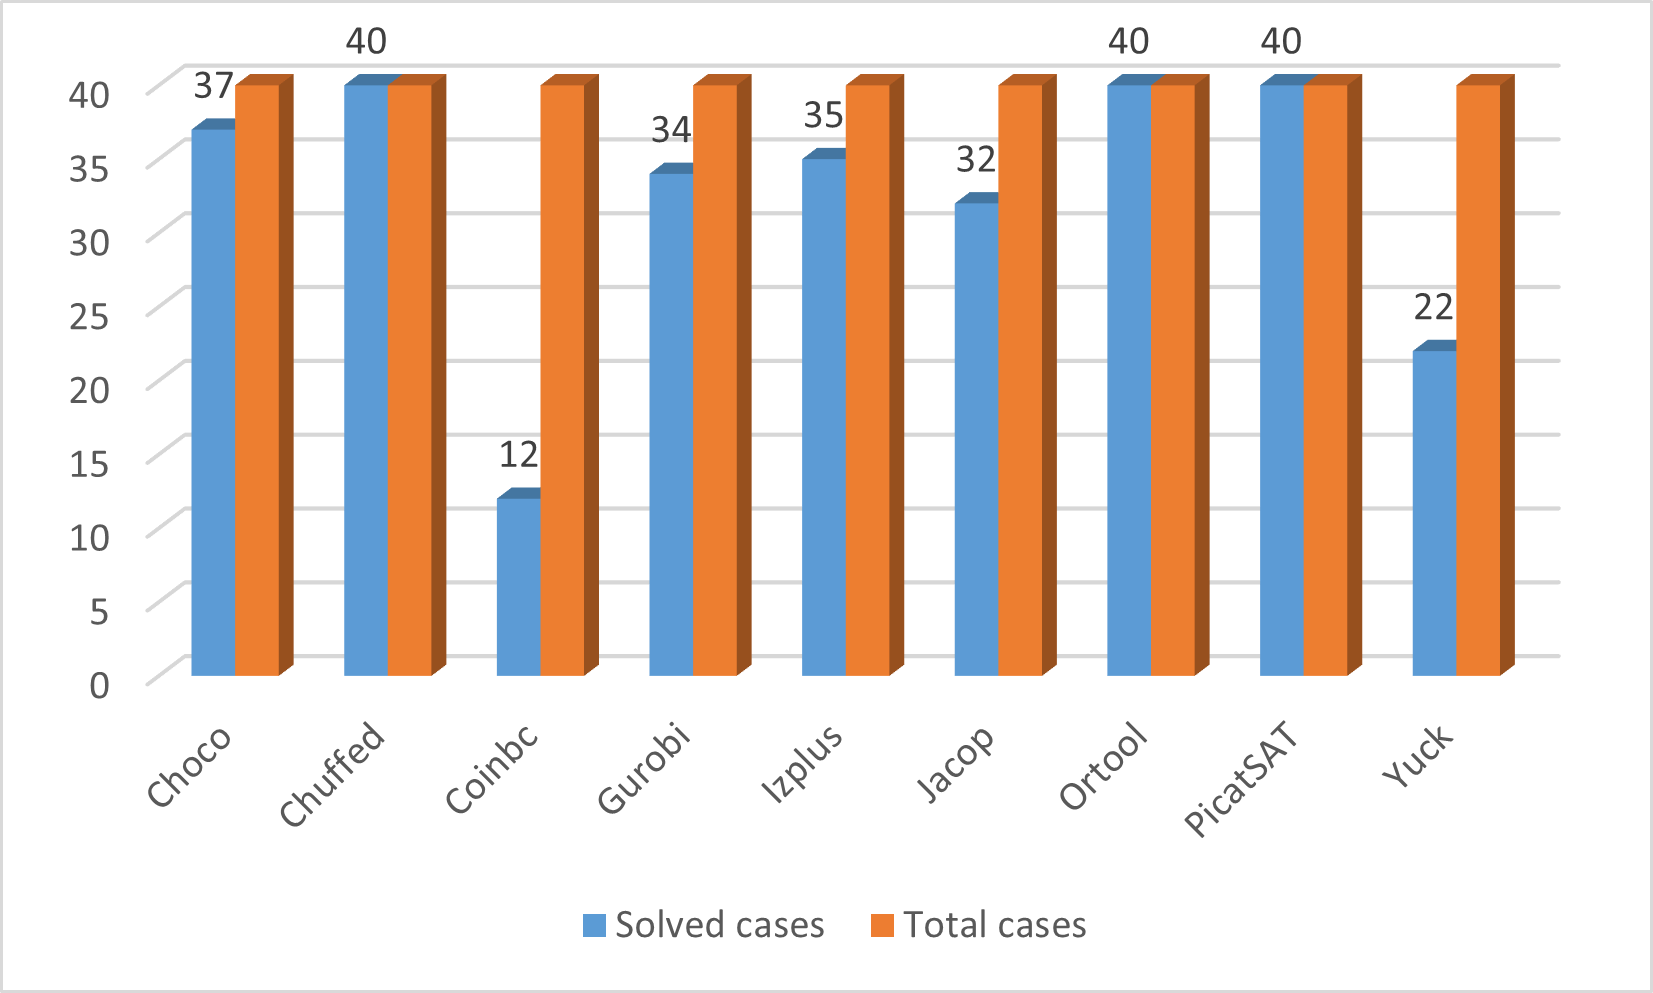
\includegraphics[width=\textwidth]{figs/mode2solvedcases.png}
    \caption{The number of solved cases of each solver}
    \label{fig:mode2eva1}
    \end{subfigure}
     \begin{subfigure}[b]{0.48\textwidth}
     \centering
    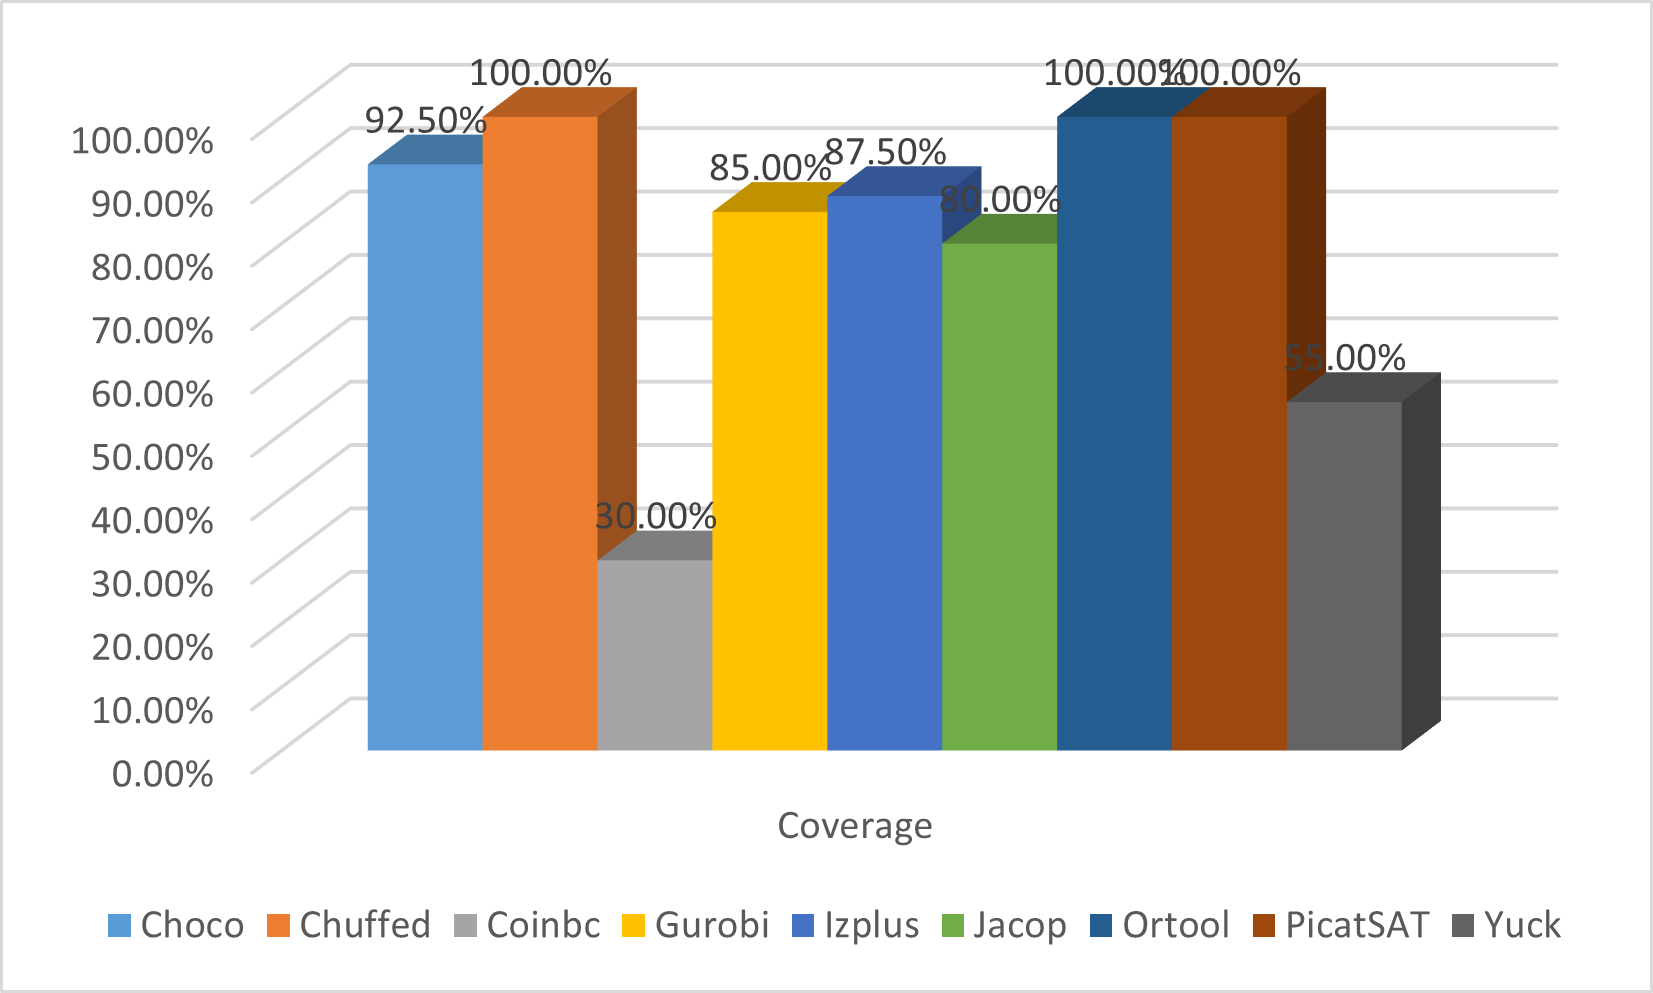
\includegraphics[width=\textwidth]{figs/mode2coverage.png}
    \caption{Overall coverage rates of each solver}
    \label{fig:mode2eva2}
    \end{subfigure}
     \begin{subfigure}[b]{0.48\textwidth}
    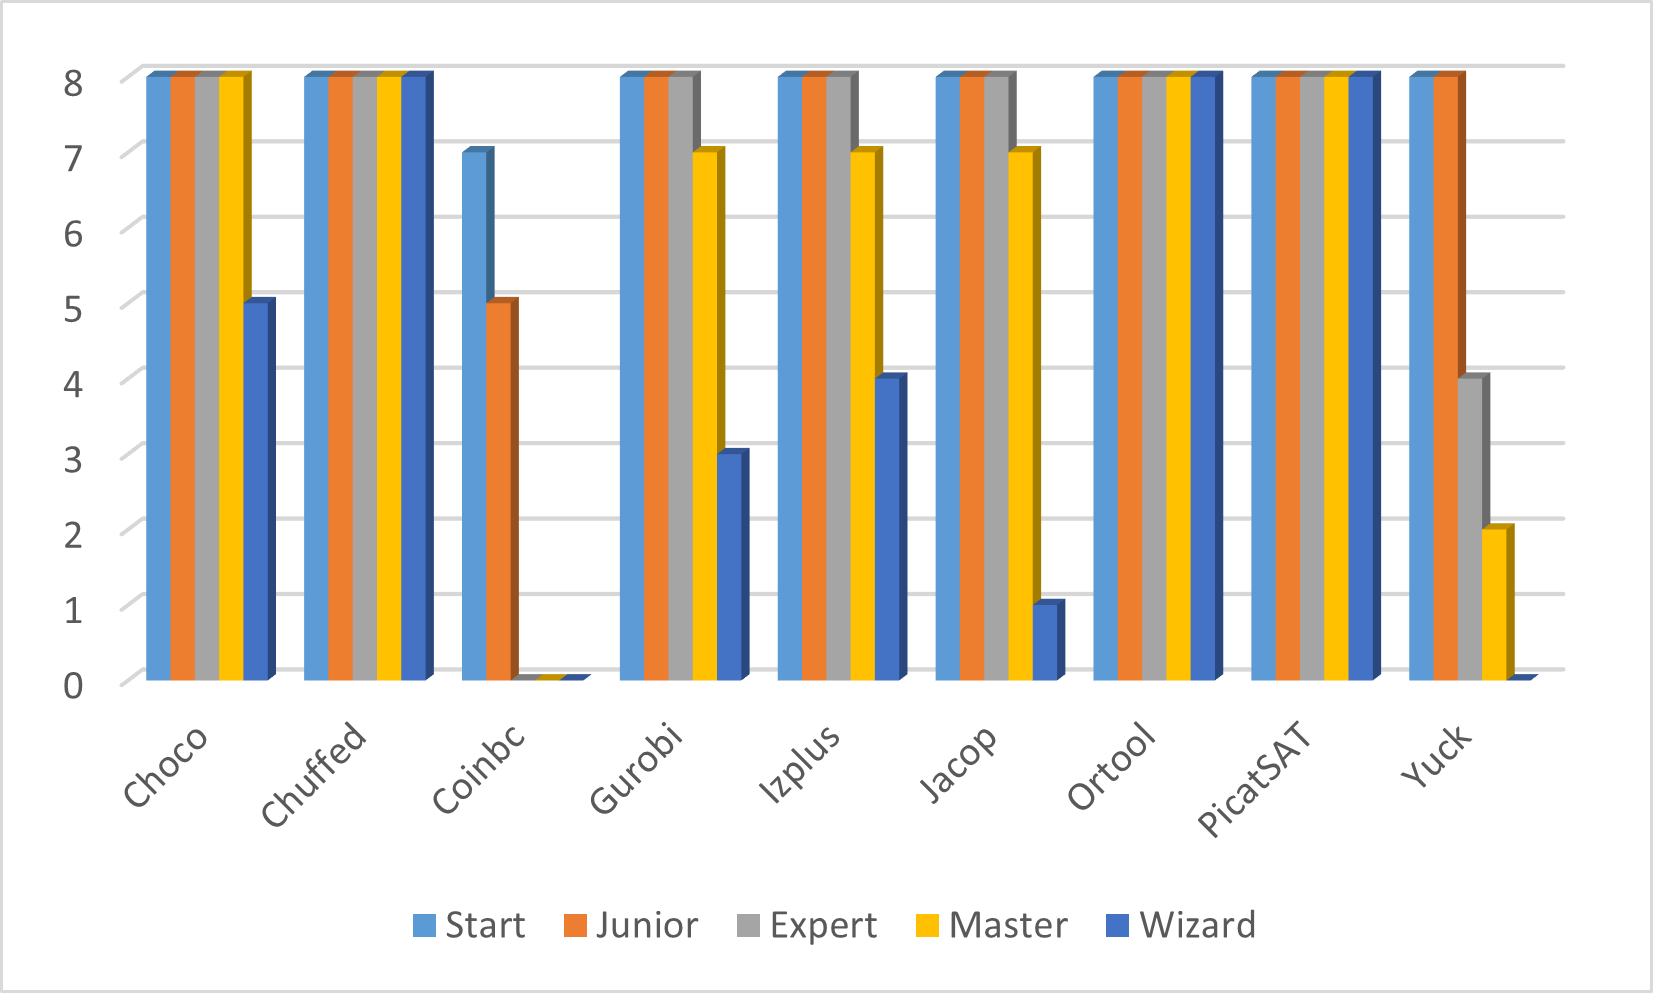
\includegraphics[width=\textwidth]{figs/mode2separatedcases.png}
    \caption{The number of solved cases of each solver for different difficulties}
    \label{fig:mode2eva3}
    \end{subfigure}
    \begin{subfigure}[b]{0.48\textwidth}
    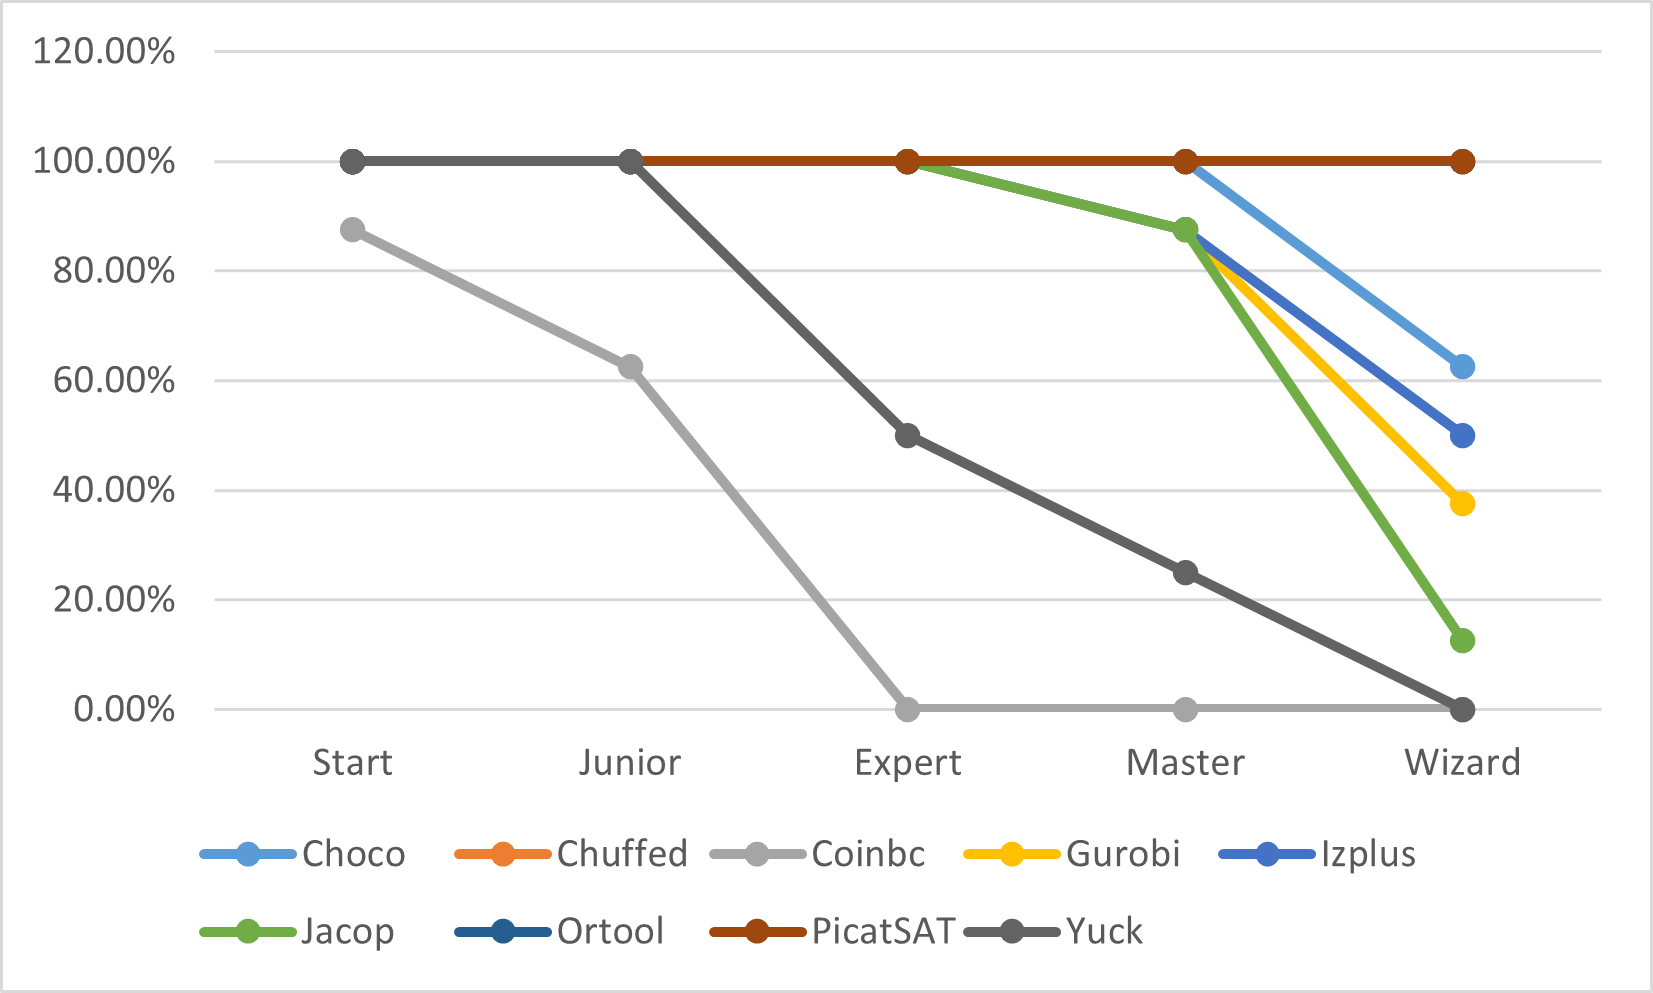
\includegraphics[width=\textwidth]{figs/mode2seperatedcoverage.png}
    \caption{The coverage rates of each solver for different difficulties}
    \label{fig:mode2eva4}
    \end{subfigure}
    \caption{Coverage rates and the number of solved cases in Zig Zag Puzzler playing mode2}
    \label{fig:comparisonmode2}
\end{figure}
As is shown in Figure~\ref{fig:comparisonmode2}, the result of coverage is quite similar with the result of coverage in playing mode 1. Chuffed, picatSAT and ortool solve each cases in 30 minutes. Meanwhile, Figure~\ref{fig:mode2eva4} the other 6 solvers' separated coverage are decreased as the difficulty increase.
For the average execution time, except yuck, all the other solvers' average execution times are positive correlation with the difficulties. Again, chuffed achieve the optimal performance. 
Similarly, Figure~\ref{fig:mode2averagetime} 
\begin{figure}[htbp]
\centering
\begin{subfigure}{0.48\textwidth}
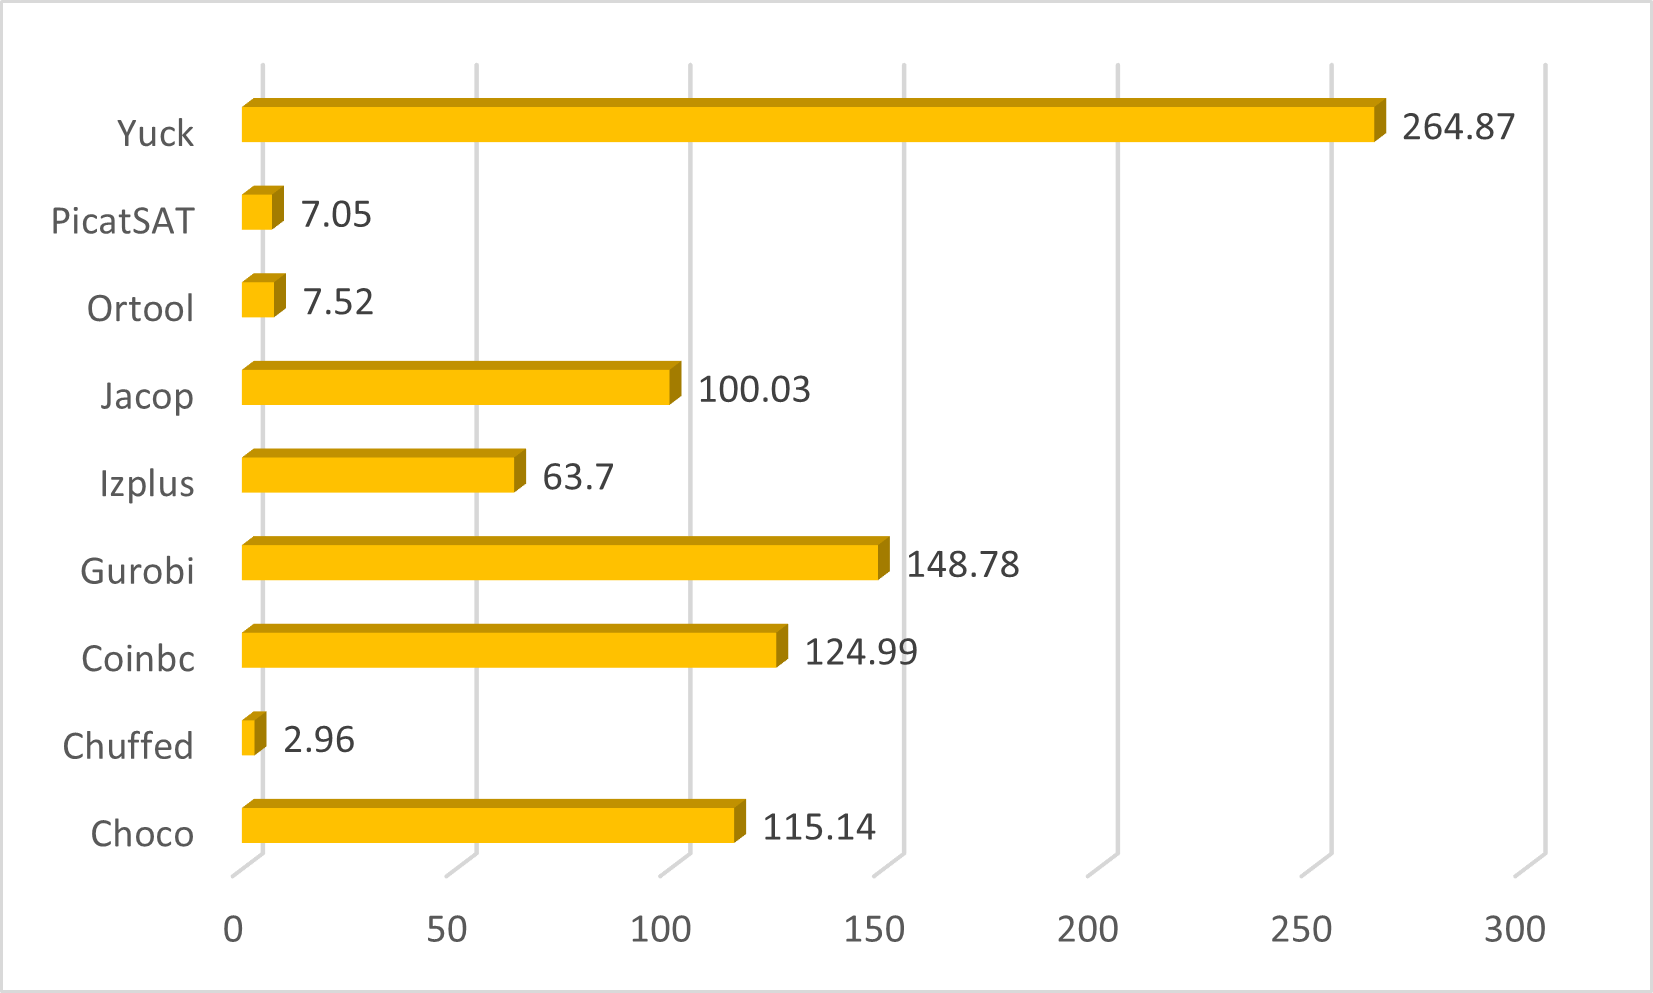
\includegraphics[width=\textwidth]{figs/mode2averagetime.png}
\caption{The overall average execution time of solved cases}
\label{fig:mode2averagetime1}
\end{subfigure}
\begin{subfigure}{0.48\textwidth}
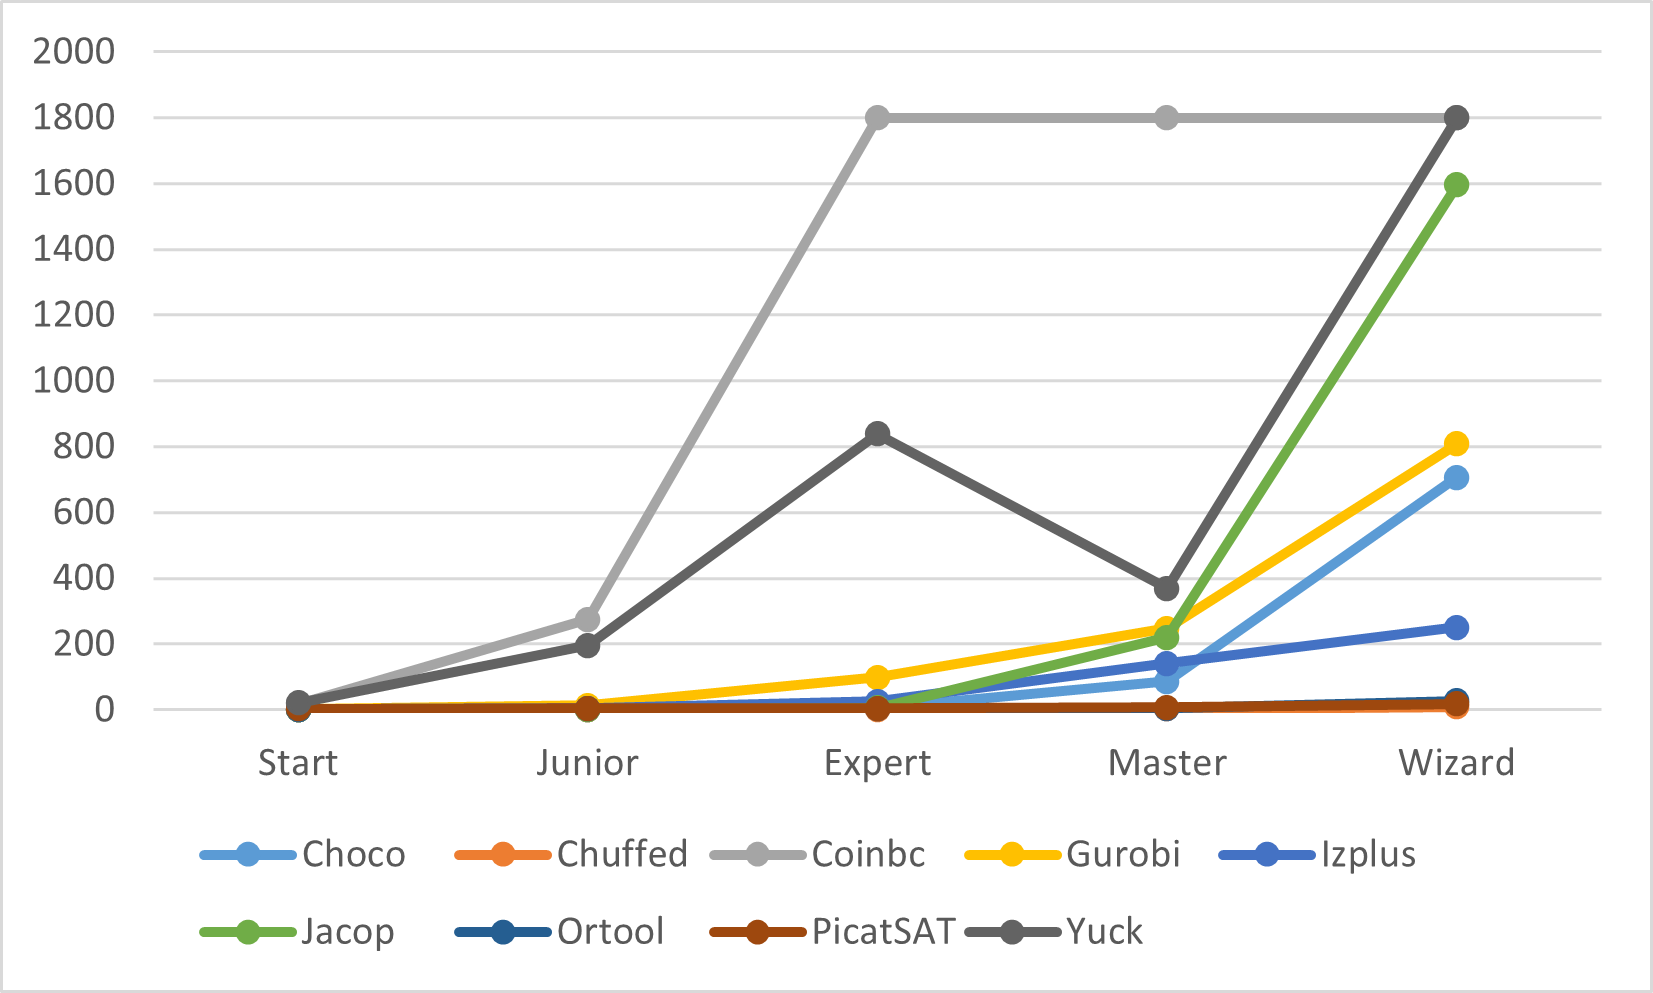
\includegraphics[width=\textwidth]{figs/mode2separatedtime.png}
\caption{The separated average execution time of solved cases}
\label{fig:mode2averagetime2}
\end{subfigure}
\caption{The average execution time of solved cases}
\label{fig:mode2averagetime}
\end{figure}

\begin{figure}[htbp]
    \centering
    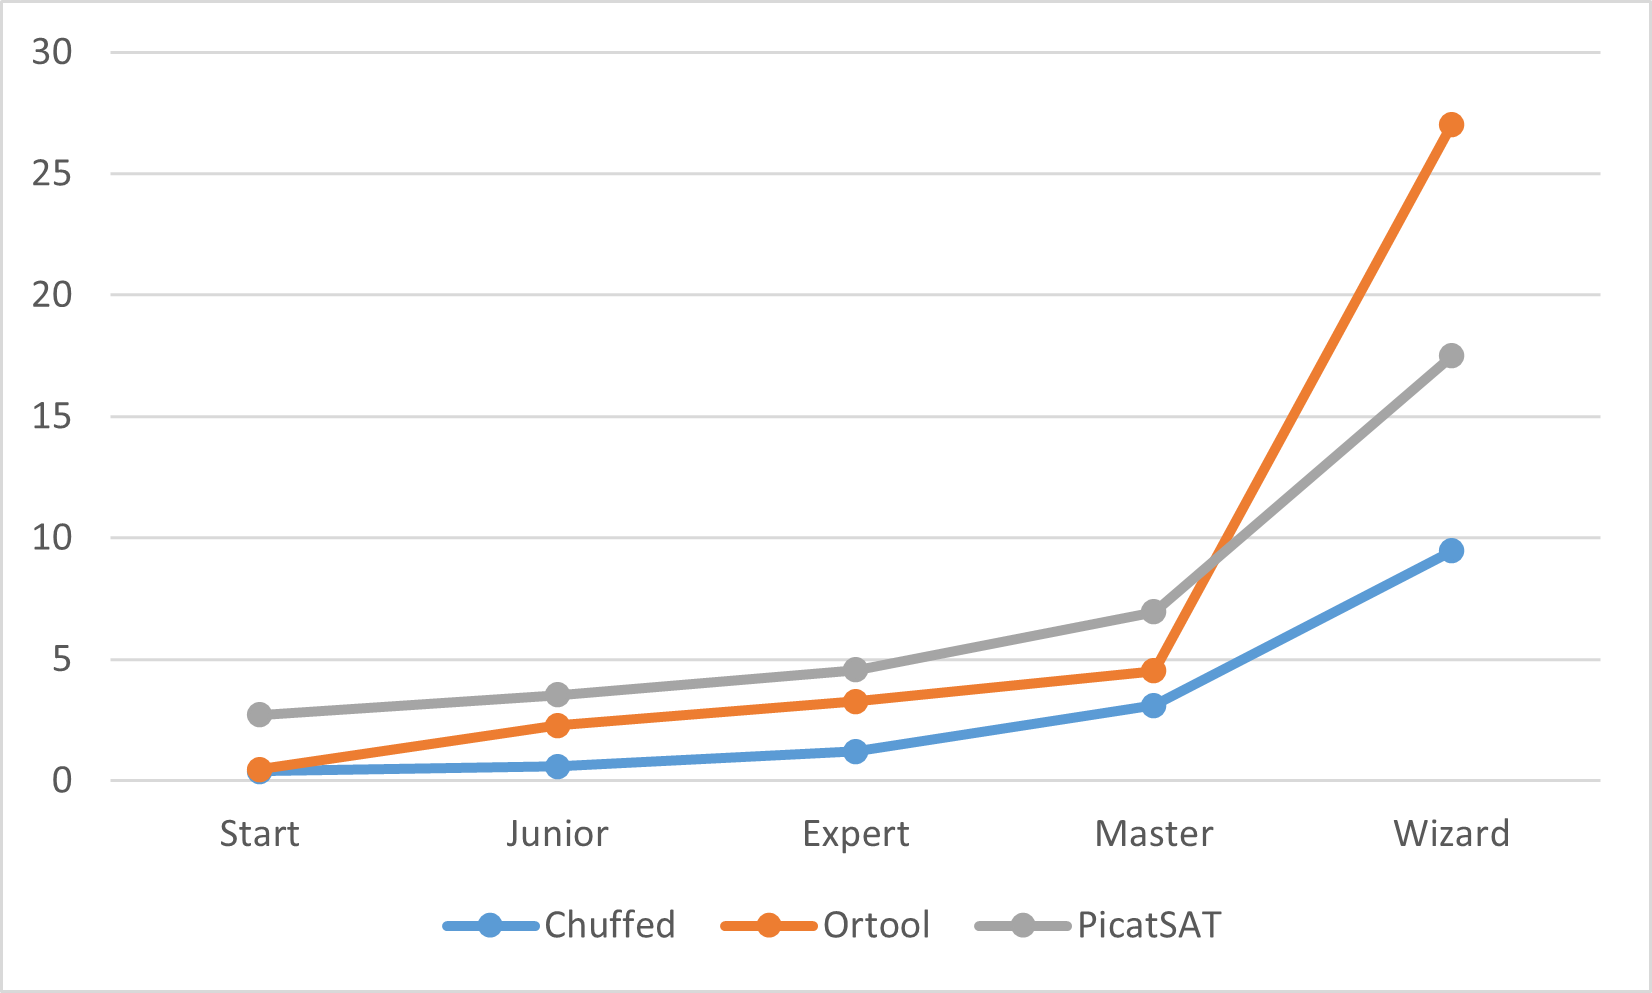
\includegraphics[width=0.6\textwidth]{figs/Threecomparison2.png}
    \caption{The separated average execution time of solved cases for chuffed, ortool and picatSAT}
    \label{fig:compare}
\end{figure}